\documentclass[11pt]{amsart}
%\documentclass[11pt]{article}
\usepackage{geometry}                % See geometry.pdf to learn the layout options. There are lots.
%\geometry{letterpaper, width=7in, height=9in}                   % ... or a4paper or a5paper or ... 
\geometry{letterpaper, width=6.5in, height=9in}                   % ... or a4paper or a5paper or ... 
\usepackage{graphicx}
\usepackage{pdfpages}
\usepackage{amssymb}
\usepackage{epstopdf}
\usepackage{color}
\usepackage{hyperref}
\usepackage{courier}
\usepackage{listings}
%\usepackage[titles]{tocloft}
%\usepackage{showkeys}
%\usepackage{refcheck}


\usepackage{siunitx}
\usepackage{booktabs}

%% Code to break page before a section begins (some section are very short so this
%% doesn't always make sense. I'd rather break the page manually).
% \let\oldsection\section
% \renewcommand\section{\clearpage\oldsection}

\DeclareGraphicsRule{.tif}{png}{.png}{`convert #1 `dirname #1`/`basename #1 .tif`.png}
\DeclareGraphicsRule{.gif}{pdf}{.pdf}{`convert #1 `dirname #1`/`basename #1 .gif`.pdf}

   \newsavebox{\fmbox}
   \newenvironment{fmpage}[1]
     {\begin{lrbox}{\fmbox}\begin{minipage}{#1}}
     {\end{minipage}\end{lrbox}\fbox{\usebox{\fmbox}}}
     
\oddsidemargin 0in
\evensidemargin 0in

%\definecolor{MRGGreen}{rgb}{0,0.655,0.212}
\definecolor{MRGGreen}{rgb}{0, 0.350, 0.200}
\parskip 10pt
\parindent 0em

\lstset{columns=fullflexible, basicstyle=\ttfamily, xleftmargin=0.5cm, frame=tlbr,framesep=4pt, framerule=0pt}

\newcommand{\torstenversion}{0.84}
\newcommand{\stanversion}{2.17.1}

% \usepackage[nottoc]{tocbibind}
%\usepackage[colorlinks=true,linkcolor=blue]{hyperref}
%\setcounter{tocdepth}{0}

%\cftsetindents{section}{0em}{2.3em}
%\cftsetindents{subsection}{0em}{4.3em}

\begin{document}

\begin{center}

\includegraphics[height=0.75in]{graphics/logo.jpg}\\
\textcolor{MRGGreen}{\sf
\begin{tabbing}
Metrum Research Group LLC \` 2 Tunxis Road, Suite 112 \\
Phone: 860.735.7043 \` Tariffville, CT 06081 \\
billgm@metrumrg.com \` metrumrg.com \\
\end{tabbing}
}
{\Huge \textcolor{MRGGreen}{\textbf{Torsten}} \\ \ \\  \huge Torsten: A Pharmacokinetic/Pharmacodynamic Model Library for Stan \\ \ \\
User Manual \\ \ \\ \ \\ \ \\
\Large Torsten Version \torstenversion \\ for Stan Version \stanversion \\ \ \\
\large February 2018}
\end{center}

\clearpage


\tableofcontents

\pagebreak

\section*{Development Team}
Bill Gillespie \\
\texttt{billg@metrumrg.com} \\
Metrum Research Group, LLC

Yi Zhang \\
\texttt{yiz@metrumrg.com} \\
Metrum Research Group, LLC

Charles Margossian \\
\texttt{charles.margossian@columbia.edu} \\
Columbia University, Department of Statistics \\
(formerly Metrum Research Group, LLC)

\section*{Acknowledgements}

{\bf Institutions} \ \\
We thank Metrum Research Group, Columbia University, and AstraZeneca.

{\bf Funding}  \ \\
This work was funded in part by the following organizations:
\begin{itemize}
\item Office of Naval Research (ONR) contract N00014-16-P-2039
  provided as part of the Small Business Technology Transfer (STTR)
  program. The content of the information presented in this document
  does not necessarily reflect the position or policy of the
  Government and no official endorsement should be inferred.
\item Bill \& Melinda Gates Foundation
\end{itemize}

{\bf Individuals} \ \\
We thank the Stan Development Team for giving us guidance on how to
create new Stan functions and adding features to Stan's core language
that facilitate building ODE-based models.

We also thank Kyle Baron and Hunter Ford for helpful advice on coding
in C++ and using GitHub, Curtis Johnston for reviewing the User
Manual, and Yaming Su for using Torsten and giving us feedback.

\pagebreak

\section{Introduction}
%\addcontentsline{toc}{section}{Introduction}

%\subsection{Goal and Scope of the Project} \ \\ \ \\ 
Stan is an open source probabilistic programing language designed
primarily to do Bayesian data analysis \cite{carpenter2016stan}. Several of its
features make it a powerful tool to specify and fit complex
models. Notably, its language is extremely flexible and its No U-Turn
Sampler (NUTS), an adaptative Hamiltonian Monte Carlo algorithm, has
proven more efficient than commonly used Monte Carlo Markov Chains
(MCMC) samplers for complex high dimensional problems \cite{nuts}. Our
goal is to harness these innovative features and make Stan a better
software for pharmacometrics modeling. Our efforts are twofold:
\begin{enumerate}
\item We contribute to the development of new mathematical tools, such
  as functions that support differential equations based models, and
  implement them directly into Stan's core language.
\item We develop Torsten, an extension with specialized
  pharmacometrics functions.
\end{enumerate}

Throughout the process, we work very closely with the Stan Development
Team. We have benefited immensely from their mentorship, advice, and
feedback. Just like Stan, Torsten is an open source project that
fosters collaborative work. Interested in contributing? Shoot us an
e-mail and we will help you help us (\url{billg@metrumrg.com})!

Torsten is licensed under the BSD 3-clause license.

\begin{fmpage}{\textwidth}
{\bf WARNING:} The current version of Torsten is a {\em prototype}. It
is being released for review and comment, and to support limited
research applications. It has not been rigorously tested and should
not be used for critical applications without further testing or
cross-checking by comparison with other methods. \\ 
\ \\
We encourage interested users to try Torsten out and are happy to
assist. Please report issues, bugs, and feature requests on
\href{https://github.com/metrumresearchgroup/stan}{our GitHub
page}: \url{https://github.com/metrumresearchgroup/stan}.
\end{fmpage}


\subsection{Installing Torsten}  \ \\ \ \\  
Installation files are available on GitHub:\\
\url{https://github.com/metrumresearchgroup/example-models}.

There is currently no mechanism to install Torsten on top of your
version of Stan. This is still a work in progress. In the meantime, we
offer a version of Stan with Torsten built inside of it. Torsten \torstenversion{}
works with Stan \stanversion{}. Torsten is built inside the Stan and Stan-math
repositories and is agnostic to the interface. We offer support to
install Torsten with rstan and CmdStan.

\subsubsection{Intalling Torsten with rstan} To install RStan with Torsten, install the R package TorstenHeaders
(https://github.com/metrumresearchgroup/TorstenHeaders) and run
install\_torsten():
\begin{lstlisting}[mathescape=true,flexiblecolumns=true,basicstyle=\ttfamily]
> devtools::install_github('metrumresearchgroup/TorstenHeaders')
> library(torstenHeaders)
> install_torsten()
\end{lstlisting}

\subsubsection{Installing Torsten with CmdStan} You can
install the CmdStan interface with Stan and Torsten using the bash
file \texttt{setupTorsten.sh}, i.e., running \texttt{sh
  setupTorsten.sh} from the command line. Then compile CmdStan by
running the command \texttt{make build}. If multiple CPU cores are
available you can speed up the installation by adding the \texttt{-jN}
option where \texttt{N} is the number of cores to use for
installation.

\subsection{Overview} \ \\ \ \\
Torsten is a collection of Stan functions to facilitate analysis of
pharmacometric data using Stan. The current version includes:
\begin{itemize}
\item Specific linear compartment models:
  \begin{itemize}
  \item One compartment model with first order absorption
  \item Two compartment model with elimination from and first order
    absorption into central compartment
  \end{itemize}
\item General linear compartment model described by a system of
  first-order \underline{linear} Ordinary Differential Equations
  (ODEs).
\item General compartment model described by a system of first order
  ODEs
\item Mix compartment model with PK forcing function described by a
  linear one or two compartment model
\end{itemize}

The models and data format are based on
NONMEM\textregistered\footnote{NONMEM\textregistered\ is licensed and
  distributed by ICON Development Solutions.}/NMTRAN/PREDPP
conventions including:
\begin{itemize}
  \item Recursive calculation of model predictions
  \begin{itemize}
    \item This permits piecewise constant covariate values
  \end{itemize}
  \item Bolus or constant rate inputs into any compartment
  \item Handles single dose and multiple dose histories
  \item Handles steady state dosing histories
  \begin{itemize}
      \item Note: The infusion time must be shorter than the inter-dose interval.
  \end{itemize}
  \item Implemented NMTRAN data items include: TIME, EVID, CMT, AMT, RATE, ADDL, II, SS
\end{itemize}

In general, all real variables may be passed as Stan parameters. A
few exceptions apply \textit{to functions which use a numerical
  integrator} (i.e. the general and the mix compartment models). The
below listed cases present technical difficulties, which we expect to
overcome in Torsten's next release:
\begin{itemize}
  \item The RATE and TIME arguments must be fixed
  \item In the case of a multiple truncated infusion rate dosing regimen:
  \begin{itemize}
    \item The bioavailability (F) and the amount (AMT) must be fixed.
  \end{itemize}
\end{itemize}   

This library provides Stan language functions that calculate amounts
in each compartment, given an event schedule and an ODE system.
    
\subsection{Implementation details}
\begin{itemize}
\item Stan version \stanversion
\item All functions are programmed in C++ and are compatible with the
  Stan math automatic differentiation library \cite{AD}
\item All functions can be called directly in a Stan file in a manner
  identical to other built-in functions
\item One and two compartment models: hand-coded analytical solutions
\item General linear compartment models with semi-analytical solutions
  using the built-in matrix exponential function
\item General compartment models with numerical solutions using
  built-in ODE integrators in Stan. The tuning parameters of the
  solver are adjustable. The steady state solution is calculated using
  a numerical algebraic solver.
\item Mix compartment model: the PK forcing function is solved
  analytically and the forced ODE system is solved numerically.
\end{itemize}

\subsection{Development plans} \ \\ \ \\
Our current plans for future development of Torsten include the
following:
\begin{itemize}
\item Build a system to easily share packages of Stan functions
  (written in C++ or in the Stan language)
\item Allow numerical methods to handle RATE, AMT, TIME, and the
  bioavailability fraction (F) as parameters in all cases.
\item Optimize Matrix exponential functions
  \begin{itemize}
  \item Function for the action of Matrix Exponential on a vector
  \item Hand-coded gradients
  \item Special algorithm for matrices with special properties
  \end{itemize}
\item Fix issue that arises when computing the adjoint of the lag time
  parameter (in a dosing compartment) evaluated at $t_{lag} = 0$.
\item Extend formal tests
  \begin{itemize}
  \item We want more C++ Google unit tests to address cases users may
    encounter
  \item Comparison with simulations from the R package
    \textit{mrgsolve} and the software NONMEM\textregistered
  \item Recruit non-developer users to conduct beta testing
  \end{itemize}
\end{itemize}

\subsection{Updates since Torsten 0.83}
\begin{itemize}
  \item Torsten is now up to date with Stan version 2.17.1.
  \item Add piecewise linear interpolation function.
\item Add univariate integral functions.
\item Minor revisions to User Manual.
\end{itemize}

%\clearpage 

\section{Using Torsten}

The reader should have a basic understanding of how Stan works before
reading this chapter. There are excellent resources online to get
started with Stan (\url{http://mc-stan.org/documentation/}).

In this section we go through the different functions Torsten adds to
Stan. It will be helpful to apply these functions to a simple
example. We have uploaded code and data on
\url{https://github.com/metrumresearchgroup/example-models}.

The core model functions of Torsten and their arguments are summarized
in Table \ref{TorstenFunctions}.

\begin{table}[!htb] %[htdp]
\caption{Core Torsten model functions and their arguments.}
\begin{center}
\begin{minipage}{\textwidth - 1in}
\begin{tabular}{p{1.5in}cp{1.5in}p{1.5in}} 
\hline\hline
 & function & argument & parameters \\
model & name & names & in {\tt theta}\\ 
\hline
{\raggedright one compartment\\ model with first order\\ absorption} 
   & {\tt PKModelOneCpt} &  
	{\tt time}, {\tt amt}, {\tt rate}, {\tt ii}, {\tt evid}, {\tt cmt}, {\tt addl}, {\tt ss}, {\tt theta}, {\tt F}, {\tt tlag} &
	$CL$, $V_2$, $k_a$ \\
\hline
{\raggedright two compartment\\ model with first order\\ absorption}
   & {\tt PKModelTwoCpt} &  
	{\tt time}, {\tt amt}, {\tt rate}, {\tt ii}, {\tt evid}, {\tt cmt}, {\tt addl}, {\tt ss}, {\tt theta}, {\tt F}, {\tt tlag} &
	$CL$, $Q$, $V_2$, $V_3$, $k_a$ \\ 
\hline
{\raggedright general linear \\ compartment model} & {\tt linOdeModel} &  
	{\tt time}, {\tt amt}, {\tt rate}, {\tt ii}, {\tt evid}, {\tt cmt}, {\tt addl}, {\tt ss}, {\tt system}, {\tt F}, {\tt tlag} &
	NA: pass in constant rate matrix instead of {\tt theta} \\
\hline
{\raggedright general compartment \\ models} & {\tt genOdeModel\_*} &  
	{\tt ODE\_system}, {\tt nCmt}, {\tt time}, {\tt amt}, {\tt rate}, {\tt ii}, {\tt evid},
        {\tt cmt}, {\tt addl}, {\tt ss}, {\tt theta}, {\tt F}, {\tt tlag}, {\tt rel\_tol}, {\tt abs\_tol}, {\tt max\_num\_steps}  &
	Parameters that get passed to ODE system  \\
\hline
{\raggedright mix 1 compartment \\ model} & {\tt mixOde1Cpt\_*} &
       {\tt reduced\_ODE\_system}, {\tt nOde}, {\tt time}, {\tt amt}, {\tt rate}, {\tt ii}, {\tt evid},
       {\tt cmt}, {\tt addl}, {\tt ss}, {\tt theta}, {\tt F}, {\tt tlag}, {\tt rel\_tol}, {\tt abs\_tol}, {\tt max\_num\_steps} &
       $CL$, $V_2$, $k_a$, followed by the parameters that get passed to the reduced ODE system \\
\hline
{\raggedright mix 2 compartment \\ model} & {\tt mixOde2Cpt\_*} &
       {\tt reduced\_ODE\_system}, {\tt nOde}, {\tt time}, {\tt amt}, {\tt rate}, {\tt ii}, {\tt evid},
       {\tt cmt}, {\tt addl}, {\tt ss}, {\tt theta}, {\tt F}, {\tt tlag}, {\tt rel\_tol}, {\tt abs\_tol}, {\tt max\_num\_steps} &
       $CL$, $Q$, $V_2$, $V_3$, $k_a$, followed by the parameters that get passed to the reduced ODE system  
\end{tabular}
\end{minipage}
\end{center}
\label{TorstenFunctions}
\end{table}
% Table \ref{precompiledModels} contains a summary of arguments for Torsten functions.


\subsection{Example 1: Two Compartment Model} \ \\

We model drug absorption in a single patient and simulate plasma drug concentrations:
\begin{itemize}
\item Multiple Doses: 1250 mg, every 12 hours, for a total of 15 doses
\item PK: plasma concentrations of parent drug ($c$)
\item PK measured at 0.083, 0.167, 0.25, 0.5, 0.75, 1, 1.5, 2, 4, 6,
  8, 10 and 12 hours after 1st, 2nd, and 15th dose. In addition, the
  PK is measured every 12 hours throughout the trial.
\end{itemize}

The plasma concentration ($c$) are simulated according to the following equations:
\begin{eqnarray*}
\log\left(c\right) &\sim& N\left(\log\left(\widehat{c}\right),\sigma^2\right) \\
 \widehat{c} &=& f_{2cpt}\left(t, CL, Q, V_2, V_3, k_a\right) \\
  \left(CL, Q, V_2, V_3, ka\right) &=& 
	\left(5\ {\rm L/h}, 8\  {\rm L/h}, 20\  {\rm L},  70\ {\rm L}, 1.2\ {\rm h^{-1}} \right) \\
  \sigma^2 &=& 0.01
\end{eqnarray*}
and the drug concentration is given by $c = y_2/V_2$.

where the mass of drug in the central compartment ($y_2$) is obtained
by solving the system of ordinary differential equations (ODEs):
\begin{eqnarray}
  \begin{aligned}
  y_1' &= -k_a y_1 \\
  y_2' &= k_a y_1 - \left(\frac{CL}{V_2} + \frac{Q}{V_2}\right) y_2 +  \frac{Q}{V_3}  y_3  \\ 
  y_3' &= \frac{Q}{V_2} y_2 - \frac{Q}{V_3} y_3
  \end{aligned}
  \label{eq:TwoCpt}
\end{eqnarray}

The data are generated using the R package \textit{mrgsolve}
\cite{mrgsolve2017}, see \texttt{TwoCptModelSimulation.R}. We use this
example to demonstrate use of several functions in the Torsten
library.

\subsection{Linear One and Two Compartment Model Function} \ \\

The one and two compartment model functions have the form:

\begin{lstlisting}[mathescape=true,flexiblecolumns=false,basicstyle=\ttfamily]
<model name>(time, amt, rate, ii, evid, cmt, addl, ss,
             theta,  F, tlag)
\end{lstlisting}

There is no need to skip a line, but we do so to distinguish between
\textit{event} arguments and \textit{model} arguments.

The event arguments describe the event schedule of the clinical
trial. \texttt{time}, \texttt{amt}, \texttt{rate}, and \texttt{ii} are
arrays of real and \texttt{evid}, \texttt{cmt}, \texttt{addl}, and
\texttt{ss} arrays of integers. All arrays have the same length, which
corresponds to the number of events.

Next we have the model arguments: \texttt{theta} contains the ODE
parameters, \texttt{F} the bioavailability fraction in each
compartment, and \texttt{tlag} the
lag time in each compartment.  The model arguments may be either one
or two dimensional arrays. If they are one dimensional arrays, the
parameters are constant for all events. If they are two dimensional
arrays then each row contains the parameters for the interval
[\texttt{time[i-1], time[i]}]. The number of rows should equal the
number of events.

The options for \textit{model name} are:
\begin{itemize}
\item PKModelOneCpt
\item PKModelTwoCpt
\end{itemize}
which respectively correspond to the one and two compartment model
with a first order absorption (Figure~\ref{cptModels}). An array in
\texttt{theta} is expected to contain parameters $CL$, $V_2$, and $ka$
for the one compartment case, and $CL$, $Q$, $V_2$, $V_3$, and $ka$
for the two compartments case, \underline{in this order}. Setting $ka$
to 0 eliminates the first-order absorption. \texttt{F} contains the
bioavailability fraction of each compartment (non-effective if set to
1) and \texttt{tlag} the lag time in each compartment (non-effective
if set to 0).

\begin{figure}[htbp]
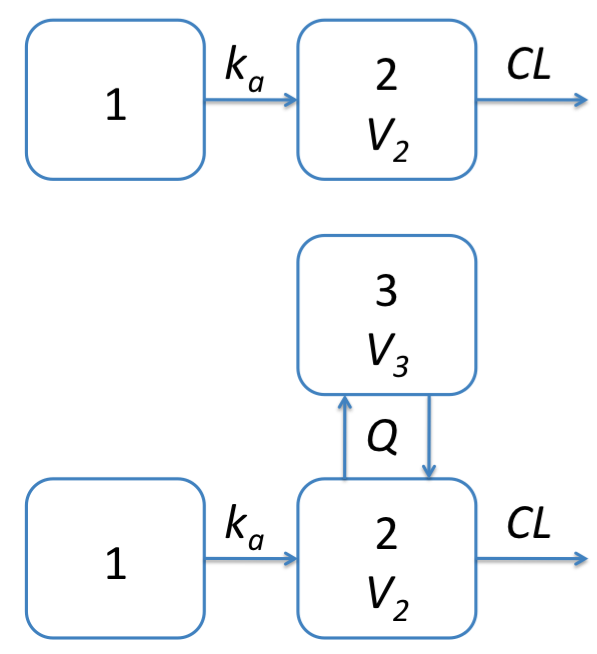
\includegraphics[width=3.5in,trim=0in 0in 0 0in]{graphics/cptModels.png}
\caption{One and two compartment models with first order absorption implemented in Torsten.}
\label{cptModels}
\end{figure}

\texttt{PKModelTwoCpt} can be used to fit example 1 as shown in Figure
\ref{TwoCptCode} and 
\texttt{TwoCptModel.stan}. We are interested in evaluating the ODE
parameters, stored in \texttt{theta}. The bioavailability fraction and
the lag times on the other hand are fixed, and we therefore declare
\texttt{F} and \texttt{tlag} in the \textbf{transformed data}
block. Three MCMC chains of 2000 iterations were simulated. The first
1000 iteration of each chain were discarded. Thus 1000 MCMC samples
per chain were used for the subsequent analyses.

\begin{figure}[htbp]
\begin{center}
\begin{small}
\begin{fmpage}{\textwidth - .75in}
\begin{lstlisting}[basicstyle=\footnotesize\ttfamily,mathescape=true,flexiblecolumns=true,frame=single,escapeinside=`']
`\bf{data}' {
  int<lower = 1> nt; `\textcolor{gray}{// number of events}'
  int<lower = 1> nObs; `\textcolor{gray}{// number of observation}'
  int<lower = 1> iObs[nObs]; `\textcolor{gray}{// index of observation}'
  int cmt[nt];
  int evid[nt];
  int addl[nt];
  int ss[nt];
  real amt[nt];
  real time[nt];
  real rate[nt];
  real ii[nt];
  
  vector<lower = 0>[nObs] cObs; `\textcolor{gray}{//  observed concentration (Dependent Variable)}'
}

`\bf{transformed data}' {
                                    $\vdots$
  F[1] = 1;
  F[2] = 1;
  F[3] = 1;
  
  tlag[1] = 0;
  tlag[2] = 0;
  tlag[3] = 0;                                    
                                    
                                     
}
                                    $\vdots$ 
`\bf{parameters}' {
  real<lower = 0> CL;
  real<lower = 0> Q;
  real<lower = 0> V2;
  real<lower = 0> V3;
  real<lower = 0> ka;
  real<lower = 0> sigma;
}

`\bf{transformed parameters}' {
                                    $\vdots$ 
  theta[1] = CL;
  theta[2] = Q;
  theta[3] = V2;
  theta[4] = V3;
  theta[5] = ka;

  x = `\textcolor{red}{PKModelTwoCpt}'(time, amt, rate, ii, evid, cmt, addl, ss, 
                          theta, F, tlag);

  cHat = col(x, 2) ./ V2; `\textcolor{gray}{//  get concentration in the central compartment}'
  
  cHatObs = cHat[iObs];  `\textcolor{gray}{// predictions for observed data records}'
 
 }
                                    $\vdots$ 
\end{lstlisting}
\end{fmpage}
\end{small}
\caption{Stan language for fitting a two compartment model using the \texttt{PKModelTwoCpt} function (abstract)}
\end{center}
\label{TwoCptCode}
\end{figure}

\textbf{Result.} The MCMC history plots (Figure~\ref{TwoCptMCMC})
suggest that the 3 chains have converged to common distributions for
all of the key model parameters. The fit to the plasma concentration
data (Figure~\ref{TwoCptPredictions}) are in close agreement with the
data, which is not surprising since the fitted model is identical to
the one used to simulate the data. Similarly the parameter estimates
summarized in Table \ref{TwoCptTable} and Figure \ref{TwoCptDensity}
are consistent with the values used for simulation.

\begin{figure}[htbp]
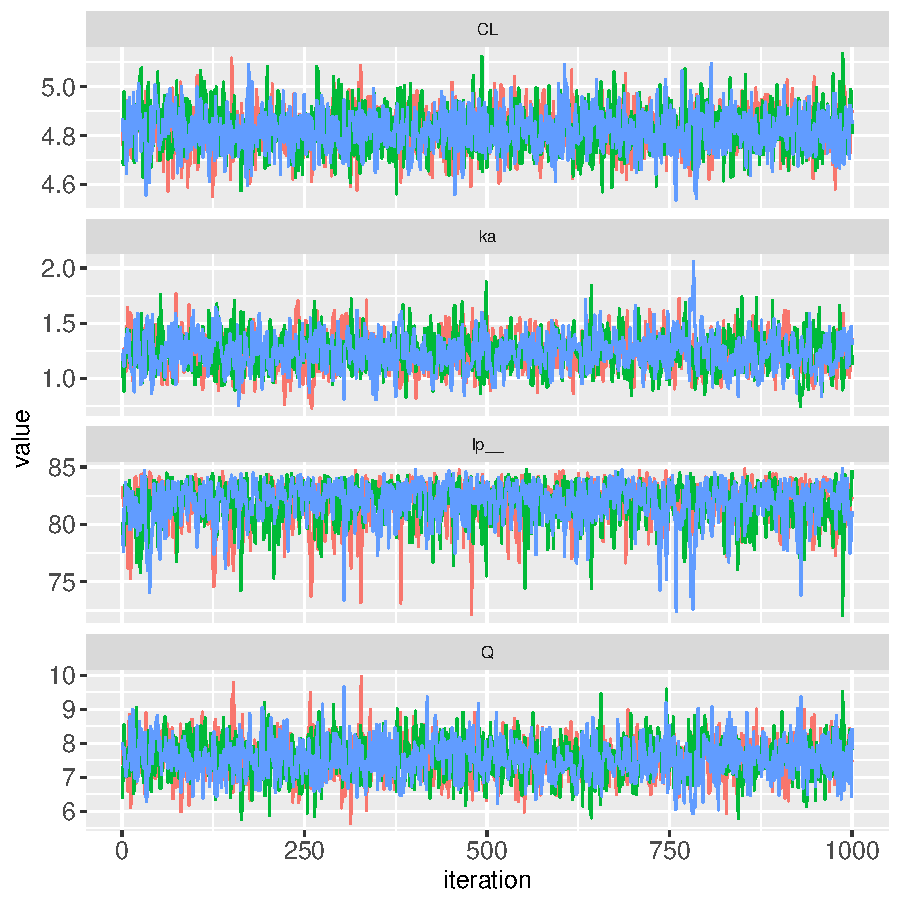
\includegraphics[width=3.0in,trim=0in 0in 0 0in]{graphics/TwoCptModelPlots001.pdf}
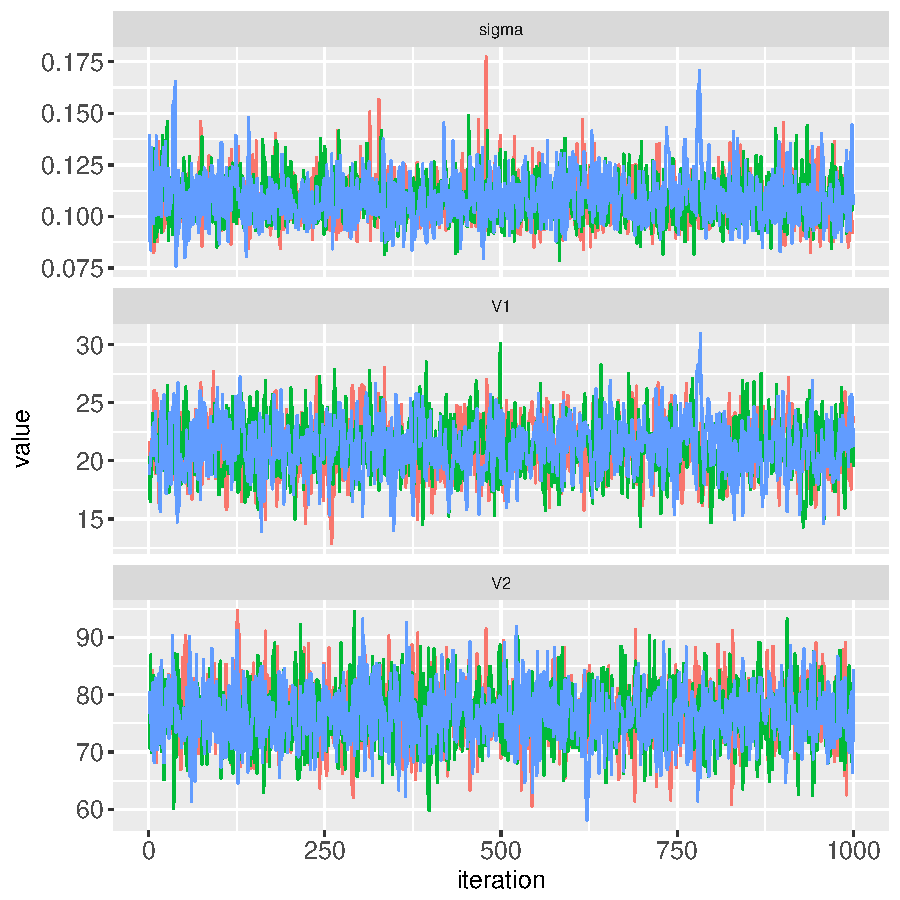
\includegraphics[width=3.0in,trim=0in 0in 0 0in]{graphics/TwoCptModelPlots002.pdf}
\caption{{MCMC history plots for the parameters of a two compartment
    model with first order absorption (each color corresponds to a
    different chain)}}
\label{TwoCptMCMC}
\end{figure}

\begin{figure}[!htb]
\begin{center}
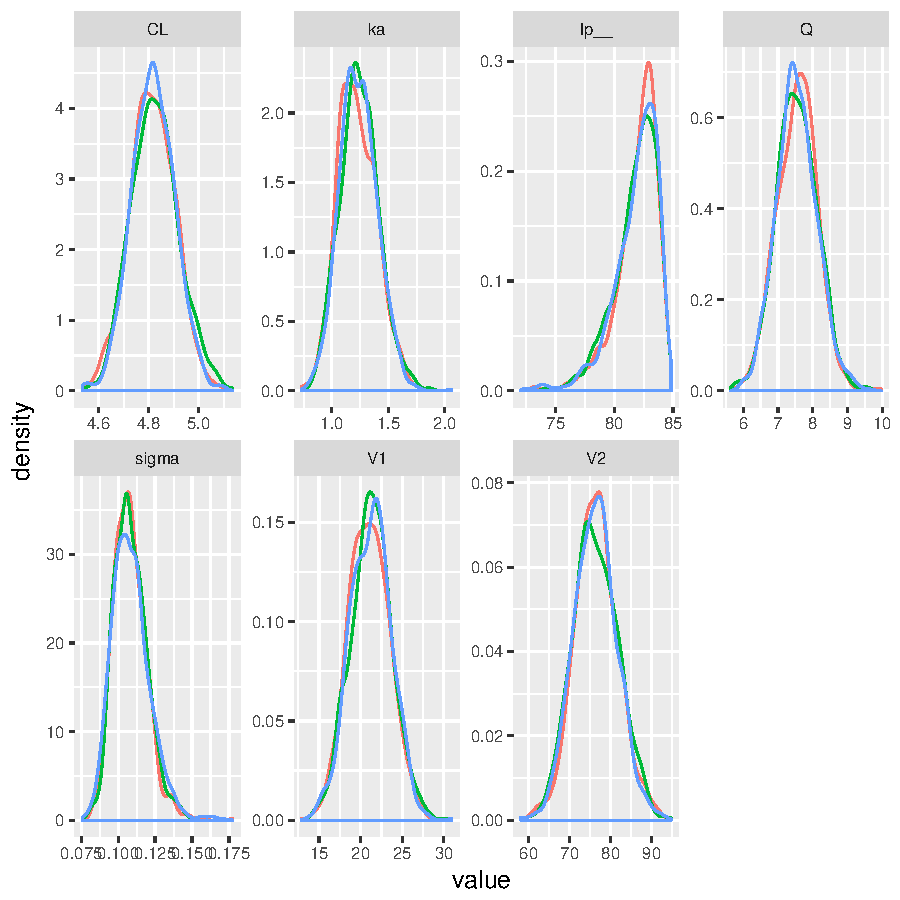
\includegraphics[width=3.5in,trim=0in 0in 0 0in]{graphics/TwoCptModelPlots003.pdf}
\caption{{Posterior Marginal Densities of the Model Parameters of a two compartment model with first order absorption (each color corresponds to a different chain)}}
\label{TwoCptDensity}
\end{center}
\end{figure}

\begin{figure}[!htb]
\begin{center}
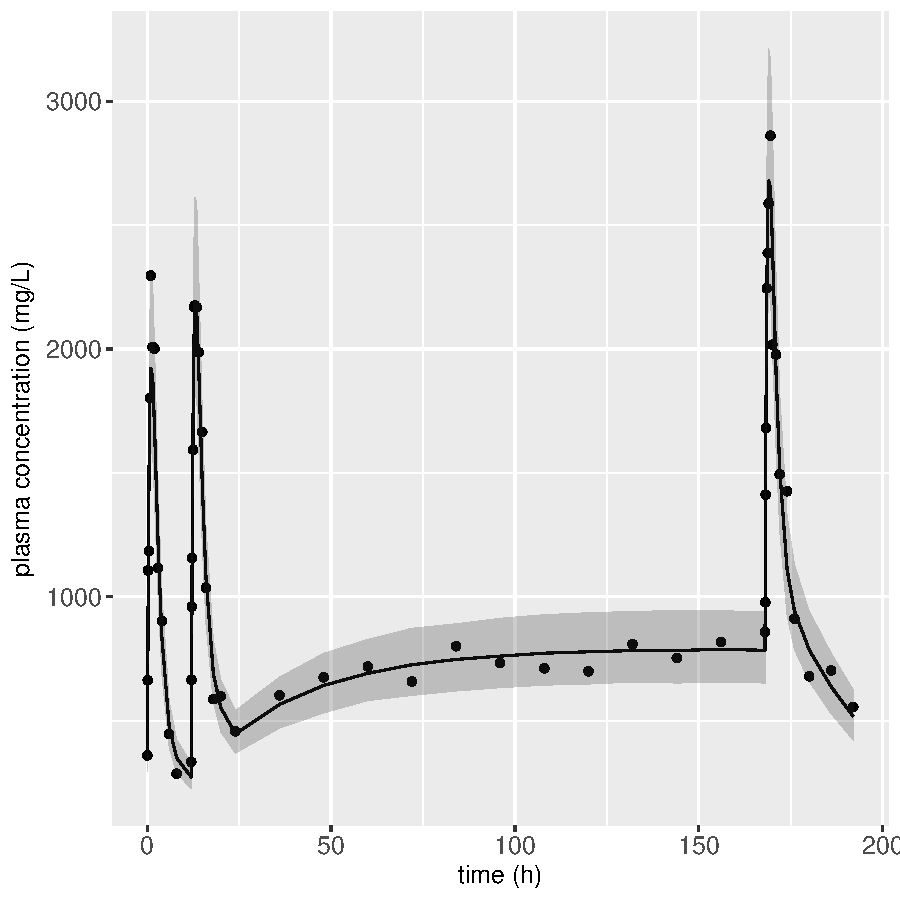
\includegraphics[width=3.5in,trim=0in 0in 0 0in]{graphics/TwoCptModelPlots006.pdf}
\caption{{Predicted (posterior median and 90 \% credible intervals) and observed plasma drug concentrations of a two compartment model with first order absorption}}
\label{TwoCptPredictions}
\end{center}
\end{figure}

\begin{table}[!htb]
\centering
\caption{Summary of the MCMC simulations of the marginal posterior
  distributions of the model parameters}
\label{TwoCptTable}
\begin{tabular}{rrrrrrrrrrr}
  \hline
 & mean & se\_mean & sd & 2.5\% & 25\% & 50\% & 75\% & 97.5\% & n\_eff & Rhat \\ 
  \hline
CL & 4.82 & 0.002 & 0.0901 & 4.64 & 4.76 & 4.82 & 4.88 & 5.00 & 2464.73 & 1.00 \\ 
  Q & 7.54 & 0.016 & 0.58 & 6.43 & 7.15 & 7.54 & 7.92 & 8.69 & 1385.75 & 1.00 \\ 
  V2 & 21.14 & 0.069 & 2.45 & 16.37 & 19.44 & 21.19 & 22.78 & 25.89 & 1245.64 & 1.00 \\ 
  V3 & 76.35 & 0.110 & 5.35 & 65.98 & 72.75 & 76.26 & 79.83 & 87.30 & 2379.15 & 1.00 \\ 
  ka & 1.23 & 0.005 & 0.169 & 0.923 & 1.12 & 1.23 & 1.35 & 1.58 & 1295.01 & 1.00 \\
  sigma & 0.108 &  0.000 & 0.012 & 0.0887 & 0.0999 & 0.107 & 0.115 & 0.135 & 1973.97 & 1.00 \\
   \hline
\end{tabular}
\end{table}

\clearpage

\subsection{General Linear ODE Model Function} \ \\

A general linear ODE model refers to a model that may be described in
terms of a system of first order linear differential equations with
(piecewise) constant coefficients, i.e., a differential equation of
the form:
$$ y^\prime\left(t\right) = Ky\left(t\right) $$ 
where $K$ is a matrix. For example $K$ for a two compartment model
(equation~\ref{eq:TwoCpt}) with first order absorption is:
$$   K = \left[\begin{array}{ccc}
	-k_a & 0 & 0 \\
	k_a & -\left(k_{10} + k_{12}\right) & k_{21} \\
	0 & k_{12} & -k_{21}
	\end{array}\right] $$
where $k_{10} = CL / V_2 $, $ k_{12} = Q / V_2 $, and $k_{21} = Q / V_3 $.

The linear ODE model function has the form:

\begin{lstlisting}[mathescape=true,flexiblecolumns=false,basicstyle=\ttfamily]
linOdeModel(time, amt, rate, ii, evid, cmt, addl, ss,
            system, F, tlag)
\end{lstlisting}

\texttt{system} can be:
\begin{itemize}
\item the matrix \texttt{K}, if the constant rate matrix is the same
  for all events.
\item an array of constant rate matrices. The length of the array is
  the number of events and each element corresponds to the matrix at
  the interval [\texttt{time[i-1], time[i]}].
\end{itemize}
\texttt{system} contains all the ODE parameters, so we no longer need
\texttt{theta}.

Figure \ref{LinTwoCptCode} and \texttt{LinTwoCptModel.stan} illustrate
the use of \texttt{linOdeModel} for fitting a two compartment model
with first order absorption.

%\clearpage

\begin{figure}[!htb]
\caption{Stan language for fitting a two compartment model using the \texttt{linOdeModel} function (abstract)}
\begin{center}
\begin{small}
\begin{fmpage}{\textwidth - .75in}
\begin{lstlisting}[basicstyle=\footnotesize\tiny\ttfamily,mathescape=true,flexiblecolumns=true,frame=single,escapeinside=`']
`\bf{transformed parameters}' {
  `\textcolor{red}{matrix[3, 3] K;}'
  real k10 = CL / V2;
  real k12 = Q / V2;
  real k21 = Q / V3;
  vector<lower = 0>[nTheta] theta[1];
  vector<lower = 0>[nt] cHat;
  vector<lower = 0>[nObs] cHatObs;
  matrix<lower = 0>[nt, 3] x;
 
  `\textcolor{red}{K = rep\_matrix(0, 3, 3);}'

  `\textcolor{red}{K[1, 1] = -ka;}'  
  `\textcolor{red}{K[2, 1] = ka;}' 
  `\textcolor{red}{K[2, 2] = -(k10 + k12);}' 
  `\textcolor{red}{K[2, 3] = k21;}' 
  `\textcolor{red}{K[3, 2] = k12;}' 
  `\textcolor{red}{K[3, 3] = -k21;}'

  x = `\textcolor{red}{linOdeModel}'(time, amt, rate, ii, evid, cmt, addl, ss,
                       K, F, tlag);

  cHat = col(x, 2) ./ V1;
  
  cHatObs = cHat[iObs];  `\textcolor{gray}{\# predictions for observed data records}'

}

`\bf{model}'{
  logCObs ~ normal(log(cHatObs), sigma);
}
\end{lstlisting}
\end{fmpage}
\end{small}
\end{center}
\label{LinTwoCptCode}
\end{figure}

\clearpage

\subsection{General ODE Model Function} \ \\

Torsten may be used to fit models described by a system of
user-specified first-order ODEs, i.e., differential equations of the form:
$$ y^\prime(t) = f(t, y(t)) $$

In the case where the rate vector $R$ is non-zero, this equation becomes:
$$ y^\prime(t) = f(t, y(t)) + R $$
  
The general ODE model functions have the form: \ \\

\begin{lstlisting}[mathescape=true,flexiblecolumns=false,basicstyle=\ttfamily]
<model\_name>(ODE\_system, nCmt,
              time, amt, rate, ii, evid, cmt, addl, ss,
              theta, F, tlag,                      
              rel\_tol, abs\_tol, max\_step)
\end{lstlisting}

where \texttt{ODE\_system} specifies $f(t, y(t))$, which the user
defines inside the \textbf{functions} block (see section 19.2 of the
Stan reference manual for details and Figure~\ref{GenTwoCptModelCode}
for an example). The user does NOT include the rates in their
definition of $f$. Torsten automatically corrects the derivatives when
the rates are non-zero.

\texttt{nCmt} is the number of compartments (or, equivalently, the
number of ODEs) in the model. \texttt{rel\_tol}, \texttt{abs\_tol},
and \texttt{max\_step} are tuning parameters for the ODE integrator:
respectively the relative tolerance, the absolute tolerance, and the
maximum number of steps.

The options for \texttt{model\_name} are:
\begin{itemize}
  \item generalOdeModel\_rk45
  \item generalOdeModel\_bdf
\end{itemize}

They respectively call the built-in Runge-Kutta 4th/5th order (rk45)
integrator, recommended for non-stiff ODEs, and the Backward
Differentiation (BDF) integrator, recommended for stiff ODEs. Which
value to use for the tuning parameters depends on the integrator and
the specifics of the ODE system. Reducing the tolerance parameters and
increasing the number of steps make for a more robust integrator but
can significantly slow down the algorithm. The following can be used
as a starting point: \mbox{\texttt{rel\_tol = 1e-6}},
\mbox{\texttt{abs\_tol = 1e-6}} and \mbox{\texttt{max\_step = 1e+6}}
for the rk45 integrator and \mbox{\texttt{rel\_tol = 1e-10}},
\mbox{\texttt{abs\_tol = 1e-10}} and \mbox{\texttt{max\_step = 1e+8}}
for the bdf integrator\footnote{These are the default tuning
  parameters for integrate\_ode\_rk45() and integrate\_ode\_bdf().
  Torsten functions do not have a default values for these
  parameters. The user must explicitly pass the tuning parameters to
  generalOdeModel\_*().}. Users should be prepared to adjust these
values. For additional information, see the Stan User's Manual
\cite[section 21.6]{stan-manual:2017}.

A few notable restrictions apply to \texttt{generalOdeModel\_*}:
\begin{itemize}
  \item \texttt{rate} and \texttt{time} cannot be passed as parameters.
  \item In the case of a multiple truncated infusion rate dosing regimen:
  \begin{itemize}
    \item The bioavailability (\texttt{F}) and the amount (\texttt{amt}) cannot be passed as parameters.
  \end{itemize}
\end{itemize}
These restrictions also apply to \texttt{mixOde\#Cpt\_*} functions, discussed in the next section.

%\clearpage

\begin{figure}
\caption{Stan language for fitting a two compartment model using the
  \texttt{generalOdeModel\_rk45} function (abstract)}
\begin{center}
\begin{small}
\begin{fmpage}{\textwidth - .75in}
\begin{lstlisting}[basicstyle=\footnotesize\ttfamily,mathescape=true,flexiblecolumns=true,frame=single,escapeinside=`']
`\bf{functions}'{
  # define ODE system for two compartment model
  real[] `\textcolor{red}{twoCptModelODE}'(real t,
			       real[] y,
			       real[] theta,
			       real[] dummy_real,
			       int[] dummy_int){
    real Q = theta[1];
    real CL = theta[2];
    real V2 = theta[3];
    real V3 = theta[4];
    real ka = theta[5];
    real k12 = Q / V2;
    real k21 = Q / V3;
    real k10 = CL / V2;
    real y[3]; 

    dydt[1] = -ka * y[1];
    dydt[2] = ka * y[1] - (k10 + k12)*y[2] + k21*y[3];
    dydy[3] = k12 * y[2] - k21 * y[3];

    return dydt;
  }
}
                                    $\vdots$
`\bf{transformed parameters}' {
                                    $\vdots$
  theta[1] = CL;
  theta[2] = Q;
  theta[3] = V1;
  theta[4] = V2;
  theta[5] = ka;

  x = `\textcolor{red}{generalCptModel\_rk45}'(`\textcolor{red}{twoCptModelODE}', 3,
                                  time, amt, rate, ii, evid, cmt, addl, ss,
                                  theta, F, tlag, 
                                  1e-8, 1e-8, 1e8);
                                    $\vdots$
\end{lstlisting}
\end{fmpage}
\end{small}
\end{center}
\label{GenTwoCptModelCode}
\end{figure}

\clearpage

\subsection{Mixed ODE Model Function} \ \\

In certain cases, an ODE system can be divided in two subsystems:

\begin{eqnarray*}
  y_1^\prime &=& f_1(t, y_1) \\
  y_2^\prime &=& f_2(t, y_1, y_2)
\end{eqnarray*} 
where $y_1$, $y_2$, $f_1$, and $f_2$ are vector-valued functions, and
$y_1^\prime$ is independent of $y_2$. This structure arises in PK/PD
models, where $y_1$ describes a forcing PK function and $y_2$ the PD
effects. If $y_1$ has an analytical solution, we can construct a
\textit{mixed solver}, which analytically solves $y_1$ and numerically
integrates $y_2$. This approach leads to an appreciable gain in
computational efficiency. In the example of a Friberg-Karlsson
semi-mechanistic model \cite{2364}, we observe an average speedup of
$\sim 47 \pm 18 \%$ when using the mix solver in lieu of the numerical
integrator. Torsten supports the mixed solver for
cases where $y_1$ solves the ODEs for a One or Two Compartment model
with a first-order absorption.

The mix ODE model functions have the form:

\begin{lstlisting}[mathescape=true,flexiblecolumns=false,basicstyle=\ttfamily]
<model\_name>(reduced\_ODE\_system, nOde,
              time, amt, rate, ii, evid, cmt, addl, ss,
              theta, F, tlag,
              rel\_tol, abs\_tol, max\_step)
\end{lstlisting}
where \texttt{reduced\_ODE\_system} specifies the system we
numerically solve ($y_2$ in the above discussion, also called the
\textit{reduced system}) and \texttt{nOde} the number of equations in
the \underline{reduced} system. The function that defines a reduced
system has an almost identical signature to that used for a full
system, but takes one additional argument: $y_1$, the PK states,
i.e. solution to the PK ODEs (Figure~\ref{reducedODESystem}).

\begin{figure}[htbp]
\caption{Stan language for defining a reduced ODE system}
\begin{center}
\begin{small}
\begin{fmpage}{\textwidth - .75in}
\begin{lstlisting}[basicstyle=\footnotesize\ttfamily,mathescape=true,flexiblecolumns=true,frame=single,escapeinside=`']
`\bf{functions}'{
  real[] reducedODE(real t,  // time
			  real[] y,  // reduced state
			  `\textcolor{red}{real[] y1,  // PK states}'
			  real[] theta,  // parameters
			  real[] x_r,  // data (real)
			  int[] x_int) {  // data (integer)	        
                                    $\vdots$			       
  }
}
\end{lstlisting}
\end{fmpage}
\end{small}
\end{center}
\label{reducedODESystem}
\end{figure}

 Again, the user does not specify the rates. Torsten automatically
 corrects the derivatives for non-zero rates.

The options for \texttt{modelName} are:
\begin{itemize}
  \item mixOde1CptModel\_rk45
  \item mixOde1CptModel\_bdf
  \item mixOde2CptModel\_rk45
  \item mixOde2CptModel\_bdf
\end{itemize}

These four functions correspond to all the permutations we can obtain
when using a forcing One or Two Compartment function, and the
Runge-Kutta 4th/5th order (rk45) or Backward Differentiation (BDF)
integration method. The mixed ODE functions can be used to compute the
steady state solutions supported by the general ODE model functions.

Restrictions regarding which arguments may be passed as parameters for
\texttt{generalOdeModel\_*} also apply to
\texttt{mixOde\#CptModel\_*}.

We cannot apply the mixed solver to the Two Compartment example we
have been using so far. Instead, we will consider the model which
motivated the implementation of the method in the first place.

\subsection{Example 2: Friberg-Karlsson Semi-Mechanistic Model} \ \\

In this second example, we add to our two Compartment model a PD
effect, described by a system of nonlinear ODEs.

Neutropenia is observed in patients receiving an ME-2 drug. Our goal
is to model the relation between neutrophil counts and drug
exposure. Using a feedback mechanism, the body maintains the number of
neutrophils at a baseline value (Figure~\ref{FK}). While in the
patient's blood, the drug impedes the production of neutrophils. As a
result, the neutrophil count goes down. After the drug clears out, the
feedback mechanism kicks in and brings the neutrophil count back to
baseline.

{\bf Friberg-Karlsson Model for drug-induced myelosuppression ($ANC$) \cite{2364}}

\begin{eqnarray*}
  \log(ANC_i) &\sim& N(\log(Circ), \sigma^2_{ANC})  \\
  Circ &=& f_{FK}(MTT, Circ_{0}, \alpha, \gamma, c)  \\
  (MTT, Circ_{0}, \alpha, \gamma, ktr) &=& (125, 5.0, 3 \times 10^{-4}, 0.17) \\
  \sigma^2_{ANC} &=& 0.001
\end{eqnarray*}
where $c$ is the drug concentration in the blood we get from the Two
Compartment model, and $Circ$ is obtained by solving the following
system of nonlinear ODEs:

\begin{eqnarray}
  \begin{aligned}
   y_\mathrm{prol}' &= k_\mathrm{prol} y_\mathrm{prol} (1 - E_\mathrm{drug})\left(\frac{Circ_0}{y_\mathrm{circ}}\right)^\gamma - k_\mathrm{tr}y_\mathrm{prol} \\
   y_\mathrm{trans1}' &= k_\mathrm{tr} y_\mathrm{prol} - k_\mathrm{tr} y_\mathrm{trans1} \\
   y_\mathrm{trans2}' &= k_\mathrm{tr} y_\mathrm{trans1} - k_\mathrm{tr} y_\mathrm{trans2}  \\
   y_\mathrm{trans3}' &= k_\mathrm{tr} y_\mathrm{trans2} - k_\mathrm{tr} y_\mathrm{trans3}  \\
   y_\mathrm{circ}' &= k_\mathrm{tr} y_\mathrm{trans3} - k_\mathrm{tr} y_\mathrm{circ}
   \end{aligned}
   \label{eq:FK}
\end{eqnarray}
where $E_{drug}  = \alpha c$.

The ODEs specifying the Two Compartment Model
(equation~\ref{eq:TwoCpt}) do not depend on the PD ODEs
(equation~\ref{eq:FK}) and can be solved analytically by Torsten. We
therefore specify our model using a mixed solver function. We do not
expect our system to be stiff and use the Runge-Kutta 4th/5th order
integrator (Figures \ref{FK_reduced} and \ref{FK_mix2}).

\begin{figure}[htbp]
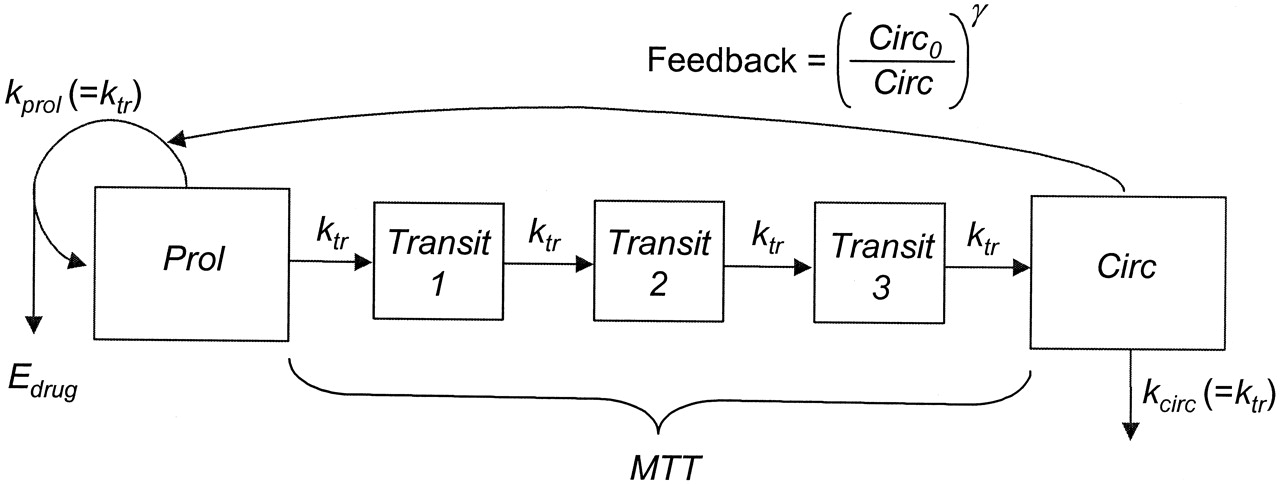
\includegraphics[width=4.5in,trim=0in 0in 0 0in]{graphics/neutrophilModel.jpg}
\caption{Friberg-Karlsson semi-mechanistic Model \cite{2364}}
\label{FK}
\end{figure}

\begin{figure}
\caption{Stan language to define a reduced ODE system}
\begin{center}
\begin{small}
\begin{fmpage}{\textwidth - .75in}
\begin{lstlisting}[basicstyle=\footnotesize\ttfamily,mathescape=true,flexiblecolumns=true,frame=single,escapeinside=`']
`\bf{functions}'{
  # define reduced ODE system for two compartment model
  real[] `\textcolor{red}{FK\_ODE}'(real t,
		    real[] y,
		    real[] y_pk,
		    real[] theta,
		    real[] dummy_real,
		    int[] dummy_int){
    real V2 = theta[3];

    ## PK variables
    real VC = parms[3];

    ## PD variables
    real MTT = parms[6];
    real circ0 = parms[7];
    real alpha = parms[8];
    real gamma = parms[9];
    real ktr = 4 / MTT;
    real prol = y[1] + circ0;
    real transit1 = y[2] + circ0;
    real transit2 = y[3] + circ0;
    real transit3 = y[4] + circ0;
    real circ = fmax(machine_precision(), y[5] + circ0);
    real conc = y_pk[2] / VC;
    real Edrug = alpha * conc;
    real dydt[5];

    conc = y_pk[2] / VC;
    Edrug = alpha * conc;

    dydt[1] = ktr * prol * ((1 - Edrug) * ((circ0 / circ)^gamma) - 1);
    dydt[2] = ktr * (prol - transit1);
    dydt[3] = ktr * (transit1 - transit2);
    dydt[4] = ktr * (transit2 - transit3);
    dydt[5] = ktr * (transit3 - circ);

    return dydt;
  }
}
\end{lstlisting}
\end{fmpage}
\end{small}
\end{center}
\label{FK_reduced}
\end{figure}

\begin{figure}
\caption{Stan language for fitting a Friberg-Karlsson model using \texttt{mixOde2CptModel\_rk45}}
\begin{center}
\begin{small}
\begin{fmpage}{\textwidth - .75in}
\begin{lstlisting}[basicstyle=\footnotesize\ttfamily,mathescape=true,flexiblecolumns=true,frame=single,escapeinside=`']
functions {
  real[] `\textcolor{red}{FK\_ODE}' {
                  $\vdots$	
  }
}

transformed date {
int `\textcolor{red}{nOde}' = 5;
                  $\vdots$
}

transformed parameters {
  vector[nt] cHat;
  vector[nObsPK] cHatObs;
  vector[nt] neutHat;
  vector<lower = 0>[nObsPD] neutHatObs;
  real theta[nParms];  # ODE parameters
  matrix[nt, nCmt] x;
  
  theta[1] = CL;
  theta[2] = Q;
  theta[3] = VC;
  theta[4] = VP;
  theta[5] = ka;
  theta[6] = mtt;
  theta[7] = circ0;
  theta[8] = alpha;
  theta[9] = gamma;

  x = `\textcolor{red}{mixOde2CptModel\_rk45}'(`\textcolor{red}{FK\_ODE}', `\textcolor{red}{nOde}',
                                   time, amt, rate, ii, evid, cmt, addl, ss,
                                   theta, F, tlag,
                                   1e-6, 1e-6, 1e+6);

  cHat = x[ , 2] / VC;
  neutHat = x[ , 8] + circ0;

  cHatObs = cHat[iObsPK];
  neutHatObs = neutHat[iObsPD];
}
\end{lstlisting}
\end{fmpage}
\end{small}
\end{center}
\label{FK_mix2}
\end{figure}

\clearpage

\subsection{Univariate integral} \ \\
Based on the ODE solver capability in Stan, Torsten is able
to calculate the integral of a univariate
function. Following the naming pattern of the ODE
solvers, the integral of function $f$ is given by

\begin{verbatim}
integral = univariate_integral_rk45(f, t0, t1, theta, x_r, x_i)
\end{verbatim}
using 4th-order Runge-Kutta integrator(for nonstiff problems), or by

\begin{verbatim}
integral = univariate_integral_bdf(f, t0, t1, theta, x_r, x_i)
\end{verbatim}
using BDF integrator(for stiff problems). Here $f$ is a
scalar-value integrand, $t0$ and $t1$ is the left and right
limit of the integral interval, respectively. $\theta$ contains 
parameters. $x_r$ and $x_i$ are real and integer data,
respectively. 

The integrand function $f$ must follow the the following
form (Figure \ref{fig:univariate_integrand}).
\begin{figure}[htbp]
\caption{Stan language for defining a univariate integrand}
\begin{center}
\begin{small}
\begin{fmpage}{\textwidth - .75in}
\begin{lstlisting}[basicstyle=\footnotesize\ttfamily,mathescape=true,flexiblecolumns=true,frame=single,escapeinside=`']
`\bf{functions}'{
  real f(real t, real[] theta, real[] x_r, int[] x_i){
                                    $\vdots$			       
  }
}
\end{lstlisting}
\end{fmpage}
\end{small}
\end{center}
\label{fig:univariate_integrand}
\end{figure}

Figure \ref{fig:univariate_int_example} shows an example using
\texttt{univariate\_integral\_rk45} to calculate the
integral of a quadratic function.
\begin{figure}[htbp]
\caption{Stan language for performing univariate integration using \texttt{univariate\_integral\_rk45}}
\begin{center}
\begin{small}
\begin{fmpage}{\textwidth - .75in}
\begin{lstlisting}[basicstyle=\footnotesize\ttfamily,mathescape=true,flexiblecolumns=true,frame=single,escapeinside=`']
`\bf{functions}'{
  real fun_ord2(real t, real[] theta, real[] x_r, int[] x_i) {
    real a = 2.3;
    real b = 2.0;
    real c = 1.5;
    real res;
    res = a + b * t + c * t * t;
    return res;
  }
}
`\bf{data}' {
  real t0;
  real t1;
  real dtheta[2];
  real x_r[0];
  int x_i[0];
}
`\bf{transformed data}' {
  real univar_integral;
  univar_integral = univariate_integral_rk45(func, t0, t1, dtheta, 
                          x_r, x_i);
}
                                    $\vdots$			       
\end{lstlisting}
\end{fmpage}
\end{small}
\end{center}
\label{fig:univariate_int_example}
\end{figure}

\subsection{Piecewise linear interpolation}\ \\ \ \\
Torsten provides a function for piecewise linear interpolation over a
set of x, y pairs. It returns the values of a piecewise linear
function at specified values ({\tt xout}) of the first function argument. The
function is specified in terms of a set of x, y pairs. The x values
must be in increasing order. All 3 arguments may be data or
parameters. 

The Stan function linear\_interpolation implements the following function.
\begin{align*}
  y_\text{out}  &= \left\{\begin{array}{ll}
                 y_1, & x_\text{out} < x_1 \\
                 y_i + \frac{y_{i+1} - y_i}{x_{i+1} - x_i}
                 \left(x_\text{out} - x_i\right), & x_\text{out} \in [x_i, x_{i+1}) \\
                 y_n, & x_\text{out} \ge x_n 
                          \end{array} \right. \\
\text{where} \\
x &= \{x_1, x_2, \ldots, x_n\} \\
y &= \{y_1, y_2, \ldots, y_n\} \\
x_{i+1} &> x_i\ \forall\ \ i
\end{align*}

The following function signatures are currently implemented:

{\tt real linear\_interpolation(real xout, real[] x, real[] y)} \\
{\tt real[] linear\_interpolation(real[] xout, real[] x, real[]
  y)} 

Use of linear\_interpolation is illustrated in a Stan model shown in
Figure \ref{linearInterpolation} for fitting a piecewise linear
function to a data set consisting of a set of x, y pairs. Complete
code for an example using that model is available on GitHub:
\url{https://github.com/metrumresearchgroup/example-models}. The
example is named testInterp2.

\begin{figure}[htbp]
\caption{Stan language model illustrating use of the
  linear\_interpolation function.}
\begin{center}
\begin{small}
\begin{fmpage}{\textwidth - .75in}
\begin{lstlisting}[basicstyle=\footnotesize\ttfamily,mathescape=true,flexiblecolumns=true,frame=single,escapeinside=`']
data{
  int nObs;
  real xObs[nObs];
  real yObs[nObs];
  int nx;
  int nPred;
  real xPred[nPred];
}

transformed data{
  real xmin = min(xObs);
  real xmax = max(xObs);
}

parameters{
  real y[nx];
  real<lower = 0> sigma;
  simplex[nx - 1] xSimplex;
}

transformed parameters{
  real yHat[nObs];
  real x[nx];

  x[1] = xmin;
  x[nx] = xmax;
  for(i in 2:(nx-1))
    x[i] = x[i-1] + xSimplex[i-1] * (xmax - xmin);

  yHat = linear_interpolation(xObs, x, y);
}

model{
  xSimplex ~ dirichlet(rep_vector(1, nx - 1));
  y ~ normal(0, 25);
  yObs ~ normal(yHat, sigma);
}

generated quantities{
  real yHatPred[nPred];
  real yPred[nPred];

  yHatPred = linear_interpolation(xPred, x, y);
  for(i in 1:nPred)
    yPred[i] = normal_rng(yHatPred[i], sigma);
}
\end{lstlisting}
\end{fmpage}
\end{small}
\end{center}
\label{linearInterpolation}
\end{figure}

\clearpage

\section{Additional Examples}

Code for examples can be found on GitHub: \url{https://github.com/metrumresearchgroup/example-models}.

All the files to run a model are stored under the directory that bears the model's name. There are four files per example:
\begin{itemize}
  \item \texttt{<model name>.stan}
  \item \texttt{<model name>.data.R}
  \item \texttt{<model name>.init.R}
  \item \texttt{<model name>Simulation.R}
\end{itemize}

\texttt{data.R} contains the data we fit the model to and \texttt{init.R} an initial estimate of the parameters. These two files are generated using \texttt{Simulation.R}. The \texttt{R} folder contains R scripts to compile and run the models, as well as code to output diagnostic plots and statistics.

\subsection {Example 3: Effect Compartment Population Model} \ \\ \ \\
Let us expand example 1 to a population model fitted to the combined data from phase I and phase IIa studies. The parameters exhibit inter-individual variations (IIV), due to both random effects and to the patients' body weight, treated as a covariate and denoted $bw$:

\subsubsection*{Population Model for Plasma Drug Concentration ($c$)}
\begin{eqnarray*}
 \log\left(c_{ij}\right) &\sim& N\left(\log\left(\widehat{c}_{ij}\right),\sigma^2\right) \\
 \widehat{c}_{ij} &=& f_{2cpt}\left(t_{ij},D_j,\tau_j,CL_j,Q_j,V_{1j},V_{2j},k_{aj}\right) \\
 \log\left(CL_j,Q_j,V_{ssj},k_{aj}\right) &\sim&
   \lefteqn{N\left(\log\left(\widehat{CL}\left(\frac{bw_j}{70}\right)^{0.75},\widehat{Q}\left(\frac{bw_j}{70}\right)^{0.75},
	\widehat{V}_{ss}\left(\frac{bw_j}{70}\right),\widehat{k}_a\right),\Omega\right)} \\
 V_{1j} &=& f_{V_1}V_{ssj} \ \ \ \ \ \ V_{2j} = \left(1 - f_{V_1}\right)V_{ssj} \\
 \left(\widehat{CL},\widehat{Q},\widehat{V}_{ss},\widehat{k}_a, f_{V_1}\right) &=& 
	\left(10\ {\rm L/h},15\  {\rm L/h},140\  {\rm L},2\ {\rm h^{-1}}, 0.25 \right) \\
\Omega &=& \left(\begin{array}{cccc} 0.25^2 & 0 & 0 & 0 \\ 0 & 0.25^2 & 0 & 0 \\
0 & 0 & 0.25^2 & 0 \\ 0 & 0 & 0 & 0.25^2  \end{array}\right), \ \ \ \sigma = 0.1 \\
\end{eqnarray*}

Furthermore we add a fourth compartment in which we measure a PD effect (Figure~\ref{effCptModel}).

\begin{figure}[htbp]
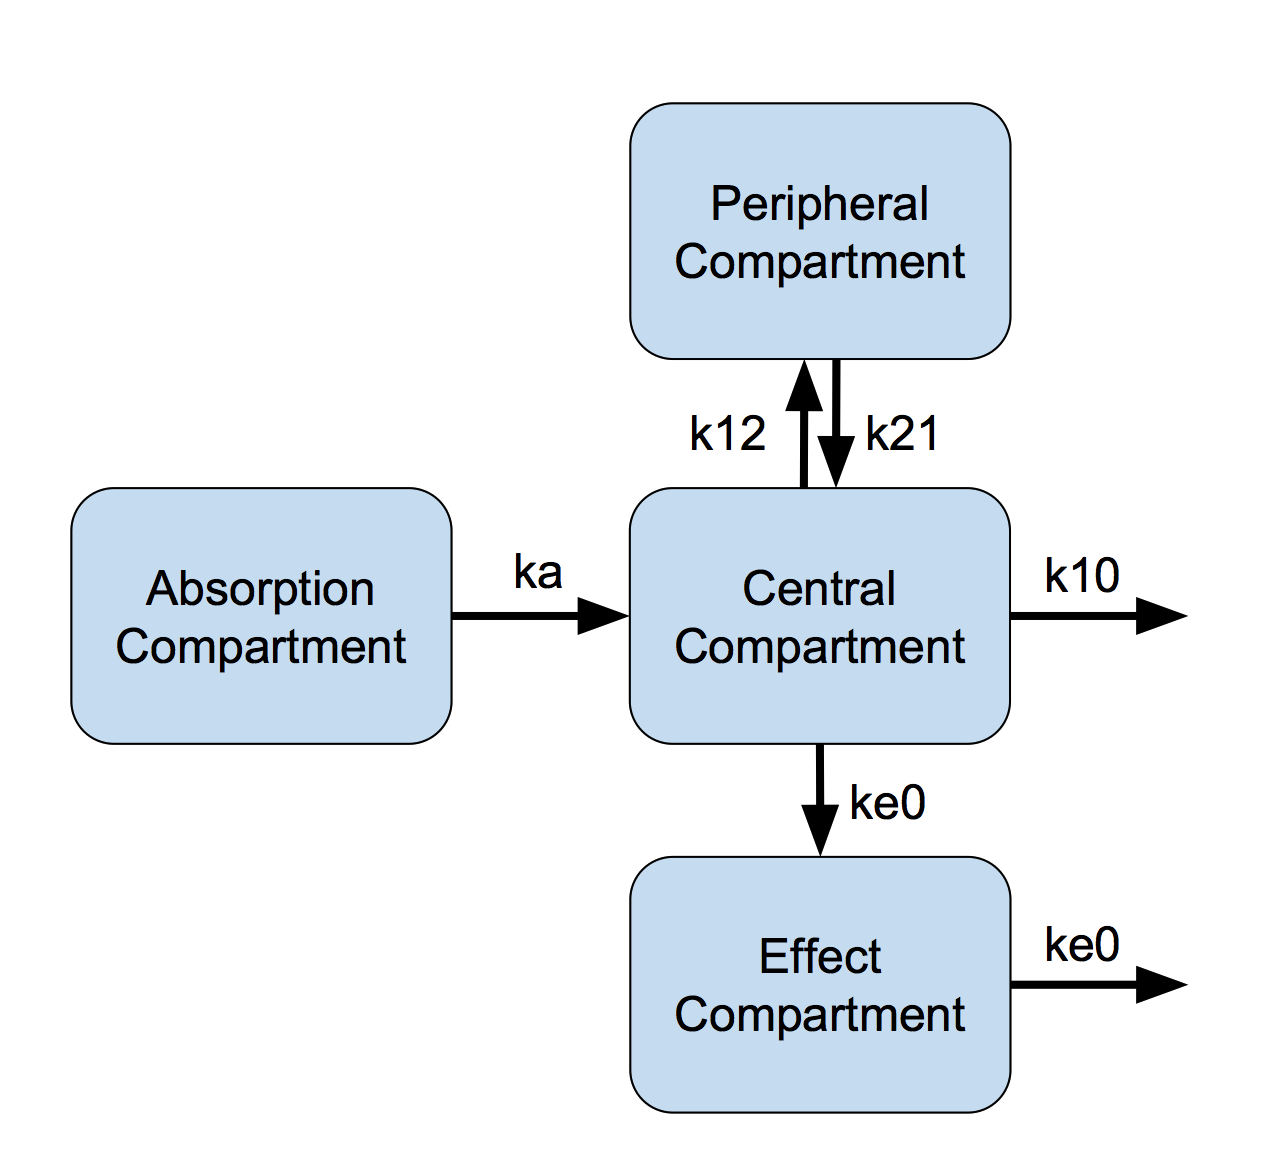
\includegraphics[width=3.5in,trim=0in 0in 0 0in]{graphics/effCptModel.png}
\caption{Effect Compartment Model}
\label{effCptModel}
\end{figure}

\subsubsection*{Effect Compartment Model for PD response ($R$)}
\begin{eqnarray*}
R_{ij} &\sim& N\left(\widehat{R}_{ij},\sigma_{R}^2\right) \\
\widehat{R}_{ij} &=& \frac{E_{max}c_{eij}}{EC_{50j} + c_{eij}} \\
c_{e\cdot j}^\prime &=& k_{e0j}\left(c_{\cdot j} - c_{e\cdot j}\right) \\
\log\left(EC_{50j}, k_{e0j}\right) &\sim& N\left(\log\left(\widehat{EC}_{50}, \widehat{k}_{e0}\right),\Omega_R\right) \\
\left(E_{max}, \widehat{EC}_{50},\widehat{k}_{e0}\right) &=& \left(100, 100.7, 1\right) \\
\Omega_R &=& \left(\begin{array}{cc} 0.2^2 & 0 \\ 0 & 0.25^2  \end{array}\right), \ \ \ \sigma_R = 10
\end{eqnarray*}

The PK and the PD data are simulated using the following treatment.
\begin{itemize}
  \item Phase I study
  \begin{itemize}
    \item Single dose and multiple doses
    \item Parallel dose escalation design
    \item 25 subjects per dose
    \item Single doses: 1.25, 5, 10, 20, and 40 mg 
    \item PK: plasma concentration of parent drug ($c$)
    \item PD response: Emax function of effect compartment concentration ($R$)
    \item PK and PD measured at 0.083, 0.167, 0.25, 0.5, 0.75, 1, 2, 3, 4, 6, 8, 12, 18, and 24 hours
  \end{itemize}
  \item Phase IIa trial in patients
  \begin{itemize}
    \item 100 subjects
    \item Multiple doses: 20 mg
    \item sparse PK and PD data (3-6 samples per patient)
  \end{itemize}
\end{itemize}

The model is simultaneously fitted to the PK and the PD data. For this
effect compartment model, we construct a constant rate matrix and use
\texttt{linOdeModel}. Correct use of Torsten requires the user pass
the entire event history (observation and dosing events) for an
individual to the function. Thus the Stan model shows the call to
\texttt{linOdeModel} within a loop over the individual subjects rather
than over the individual observations (Figure \ref{effCptModelCode}.

\begin{figure}
\caption{Stan language for fitting an effect compartment model using \texttt{linOdeModel} (abstract)}
\begin{small} 
\begin{center}
\begin{fmpage}{\textwidth - .75in}
\begin{lstlisting}[basicstyle=\tiny\ttfamily,mathescape=true,flexiblecolumns=true,frame=single,escapeinside=`']
transformed parameters {
  for(j in 1:nSubjects){
                             $\vdots$
  Omega = quad_form_diag(rho, omega);

  for(j in 1:nSubjects){
    CL[j] = exp(logtheta[j, 1]) * (weight[j] / 70)^0.75;
    Q[j] = exp(logtheta[j, 2]) * (weight[j] / 70)^0.75;
    V1[j] = exp(logtheta[j, 3]) * weight[j] / 70;
    V2[j] = exp(logtheta[j, 4]) * weight[j] / 70;
    ka[j] = exp(logtheta[j, 5]);
    ke0[j] = exp(logKe0[j]);
    EC50[j] = exp(logEC50[j]);

    k10 = CL[j] / V1[j];
    k12 = Q[j] / V1[j];
    k21 = Q[j] / V2[j];                       
    ke0[j] = exp(logKe0[j]);
    EC50[j] = exp(logEC50[j]);

    K = rep_matrix(0, 4, 4);
    
    K[1, 1] = -ka[j];
    K[2, 1] = ka[j];
    K[2, 2] = -(k10 + k12);
    K[2, 3] = k21;
    K[3, 2] = k12;
    K[3, 3] = -k21;
    K[4, 2] = ke0[j];
    K[4, 4] = -ke0[j];
           
    x[start[j]:end[j],] = `\textcolor{red}{linOdeModel}'(time[start[j]:end[j]], 
                                                 amt[start[j]:end[j]], 
                                                 rate[start[j]:end[j]],
                                                 ii[start[j]:end[j]], 
                                                 evid[start[j]:end[j]],
                                                 cmt[start[j]:end[j]], 
                                                 addl[start[j]:end[j]], 
                                                 ss[start[j]:end[j]], 
                                                 K, F, tlag);

    cHat[start[j]:end[j]] = 1000 * x[start[j]:end[j], 2] ./ V1[j];
    ceHat[start[j]:end[j]] = 1000 * x[start[j]:end[j], 4] ./ V1[j];
    respHat[start[j]:end[j]] = 100 * ceHat[start[j]:end[j]] ./ 
       (EC50[j] + ceHat[start[j]:end[j]]);
  }

  cHatObs = cHat[iObs];
  respHatObs = respHat[iObs];
}
                             $\vdots$  
} 
\end{lstlisting}
\end{fmpage}
\end{center}
\end{small}
\label{effCptModelCode}
\end{figure}

\subsubsection*{Results} We use the same diagnosis tools as for the
previous example. The MCMC history plots (Figure
\ref{effCptModelMCMC}) suggest the 4 chains have converged to common
distributions. We note some minor auto-correlations for $lp\_$ (the
log posterior) and for IIV parameters: specifically $\Omega_{ke\_0}$
and $\rho$. The correlation matrix $\rho$ does not explicitly appear
in the model, but it is used to construct $\Omega$, which parametrizes
the PK IIV. The fits to the plasma concentration
(Figure~\ref{effCptModelPredictionsPK}) are in close agreement with
the data, notably for the sparse data case (phase IIa study). The fits
to the PD data (Figure~\ref{effCptModelPredictionsPD}) look good,
though the data is more noisy. The model reflects the noise by
producing larger credible intervals. The estimated values of the
parameters are consistent with the values used to simulate the data
(Table \ref{effCptModelParms} and Figure \ref{effCptModelDens}).

\begin{table}[!htb]
\centering
\caption{Summary of the MCMC simulations of the marginal posterior
  distributions of the model parameters for the effect compartment
  model example.}
\label{effCptModelParms}
\begin{tabular}{rrrrrrrrrrr}
  \hline
 & mean & se\_mean & sd & 2.5\% & 25\% & 50\% & 75\% & 97.5\% & n\_eff & Rhat \\ 
  \hline
CLHat & 10.523 & 0.003 & 0.201 & 9.712 & 9.958 & 10.096 & 10.231 & 10.483 & 4000.000 & 0.999 \\
QHat & 14.867 & 0.014 & 0.357 & 14.182 & 14.620 & 14.862 & 15.106 & 15.563 & 678.208 & 1.007 \\
V1Hat & 34.188 & 0.067 & 1.089 & 31.940 & 33.494 & 34.214 & 34.918 & 36.251 & 267.748 & 1.016 \\
V2Hat & 103.562 & 0.076 & 2.925 & 98.031 & 101.600 & 103.455 & 105.472 & 109.583 & 488.296 & 1.001 \\
kaHat & 1.930 & 0.004 & 0.077 & 1.771 & 1.880 & 1.933 & 1.982 & 2.076 & 334.888 & 1.014 \\
ke0Hat & 1.050 & 0.001 & 0.044 & 0.967 & 1.020 & 1.051 & 1.078 & 1.137 & 164.741 & 1.000 \\
EC50Hat & 104.337 & 0.040 & 2.100 & 100.169 & 102.909 & 104.345 & 105.768 & 108.351 & 744.041 & 1.000 \\
sigma & 0.099 & 0.000 & 0.002 & 0.095 & 0.097 & 0.099 & 0.100 & 0.103 & 906.342 & 1.002 \\
sigmaResp & 10.156 & 0.003 & 0.197 & 9.779 & 10.023 & 10.154 & 10.286 & 10.552 & 4000.000 & 1.000 \\
omega[1] & 0.270 & 0.000 & 0.016 & 0.241 & 0.259 & 0.269 & 0.280 & 0.302 & 4000.000 & 1.001 \\
omega[2] & 0.231 & 0.001 & 0.021 & 0.192 & 0.217 & 0.230 & 0.245 & 0.275 & 531.512 & 1.006 \\
omega[3] & 0.219 & 0.002 & 0.031 & 0.158 & 0.199 & 0.218 & 0.238 & 0.281 & 158.198 & 1.017 \\
omega[4] & 0.267 & 0.001 & 0.026 & 0.218 & 0.249 & 0.266 & 0.284 & 0.319 & 684.870 & 1.001 \\
omega[5] & 0.285 & 0.002 & 0.037 & 0.214 & 0.259 & 0.284 & 0.309 & 0.361 & 284.545 & 1.009 \\
omegaKe0 & 0.271 & 0.003 & 0.047 & 0.183 & 0.239 & 0.271 & 0.303 & 0.363 & 217.350 & 1.007 \\
omegaEC50 & 0.213 & 0.001 & 0.021 & 0.174 & 0.199 & 0.213 & 0.227 & 0.255 & 190.193 & 1.000 \\
  \hline
\end{tabular}
\end{table}

%\clearpage

\begin{figure}[!htb]
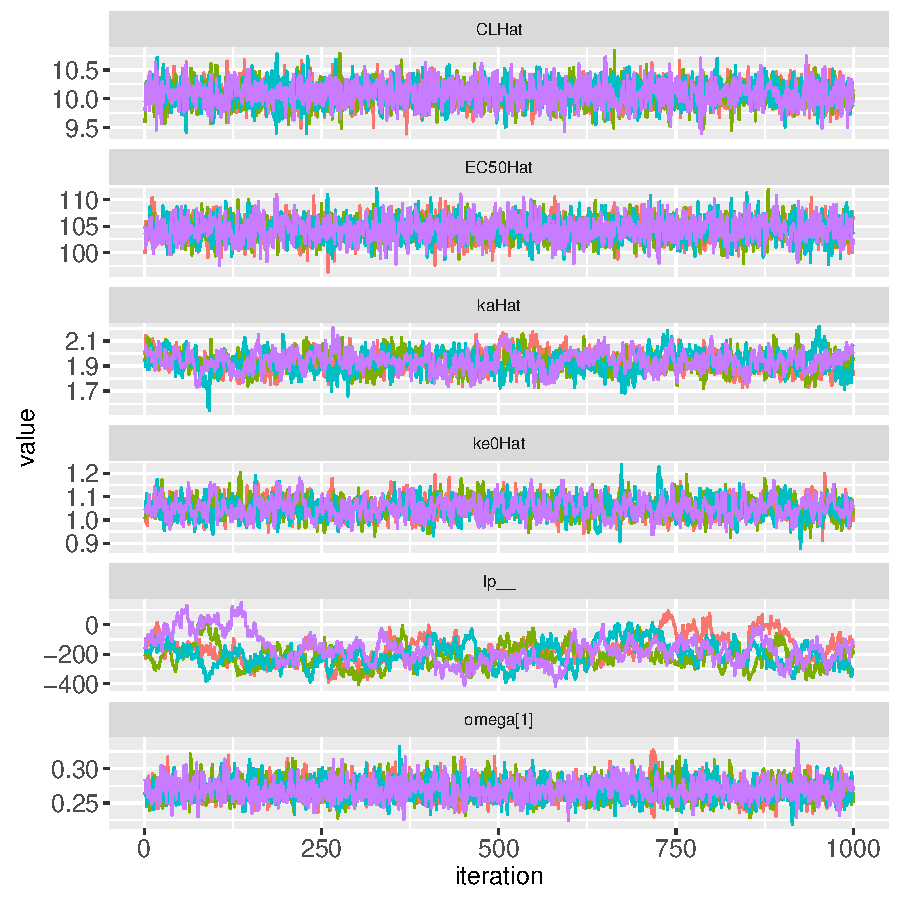
\includegraphics[width=3.0in,trim=0in 0in 0 0in]{graphics/effCptModelTorsten_0.82/effCptPlots001.pdf}
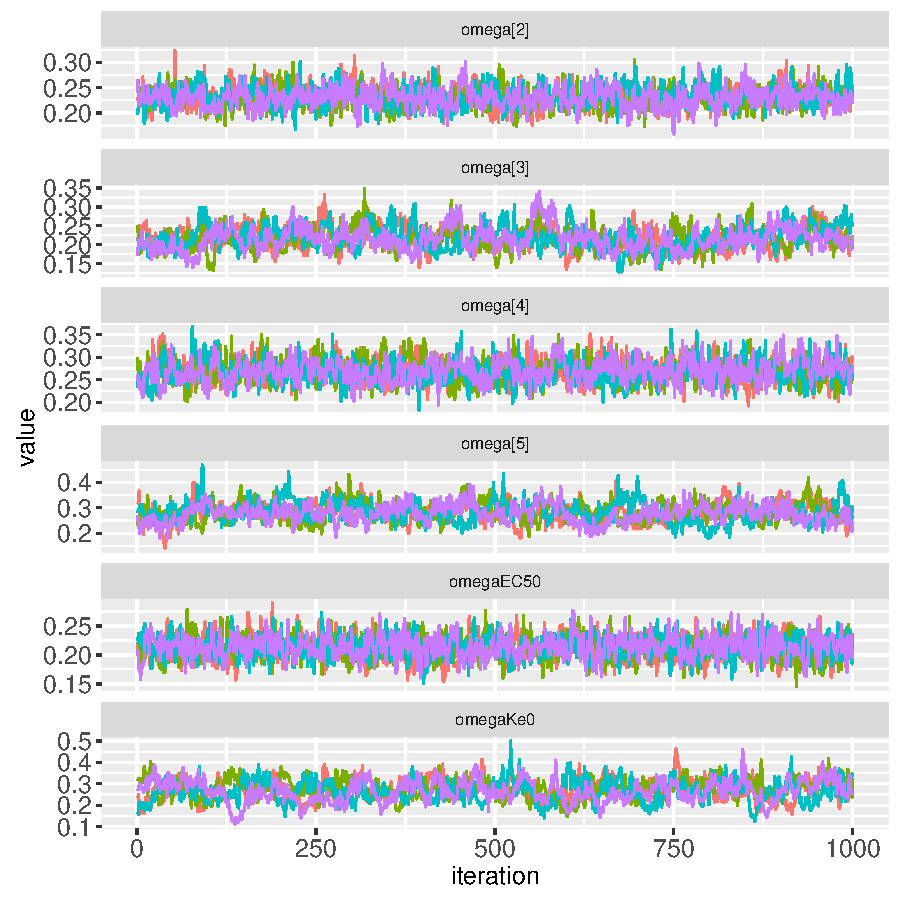
\includegraphics[width=3.0in,trim=0in 0in 0 0in]{graphics/effCptModelTorsten_0.82/effCptPlots002.pdf}
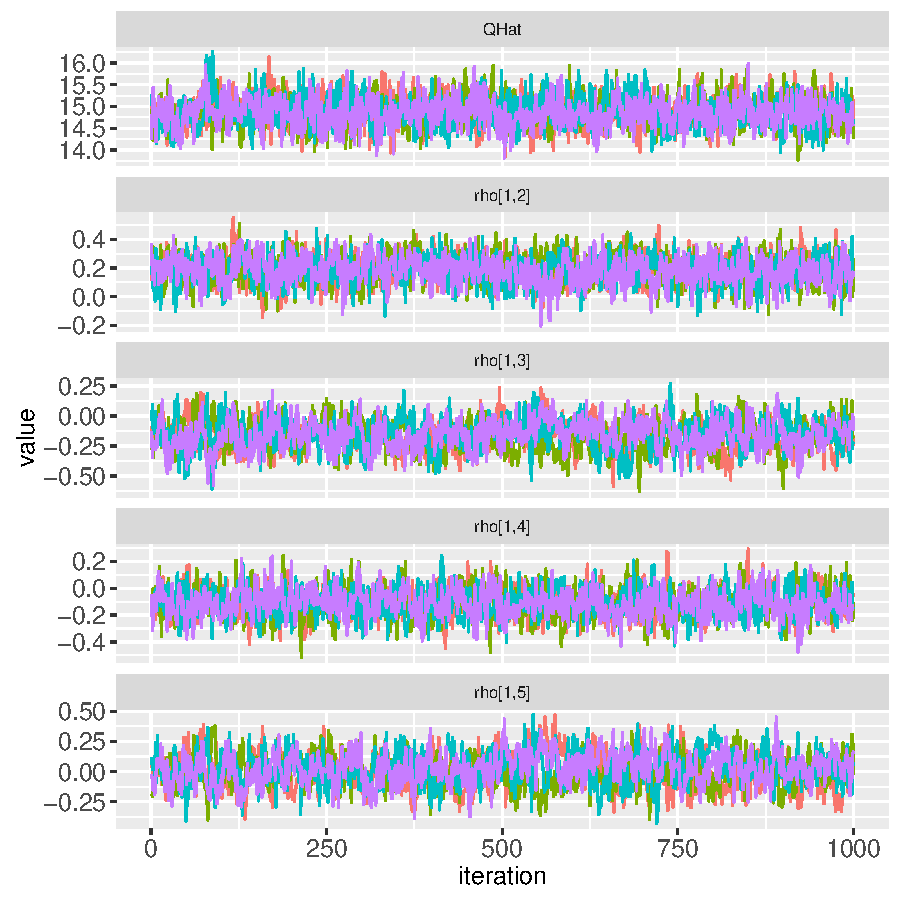
\includegraphics[width=3.0in,trim=0in 0in 0 0in]{graphics/effCptModelTorsten_0.82/effCptPlots003.pdf}
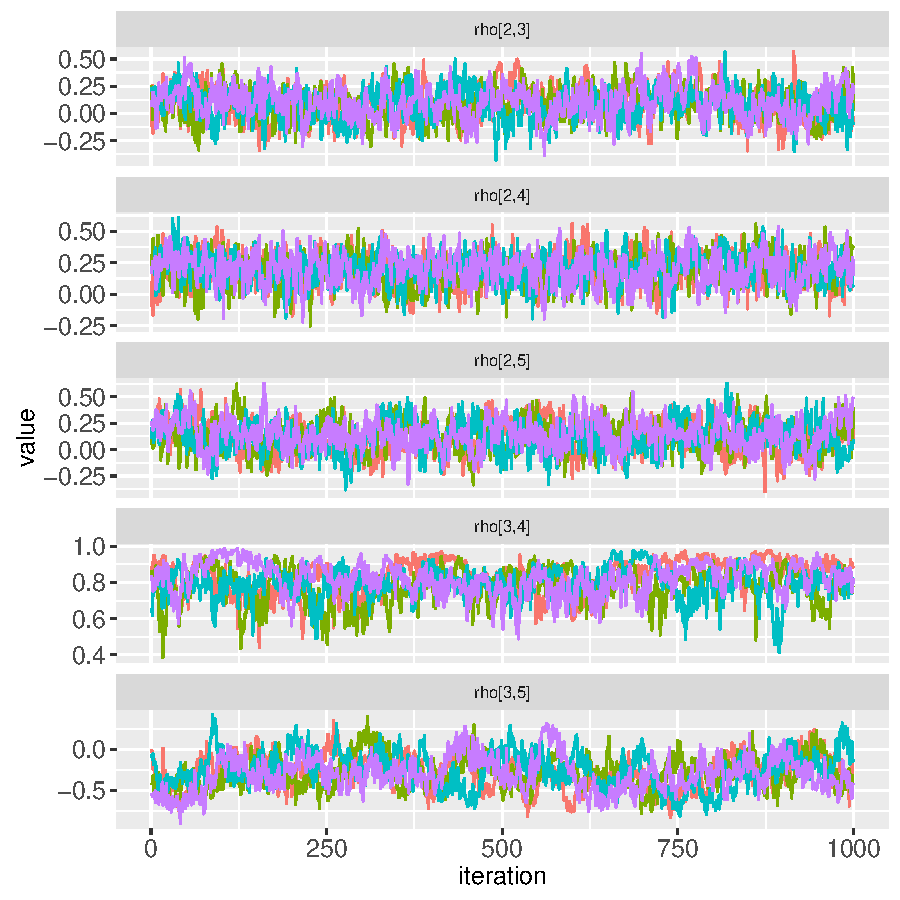
\includegraphics[width=3.0in,trim=0in 0in 0 0in]{graphics/effCptModelTorsten_0.82/effCptPlots004.pdf}
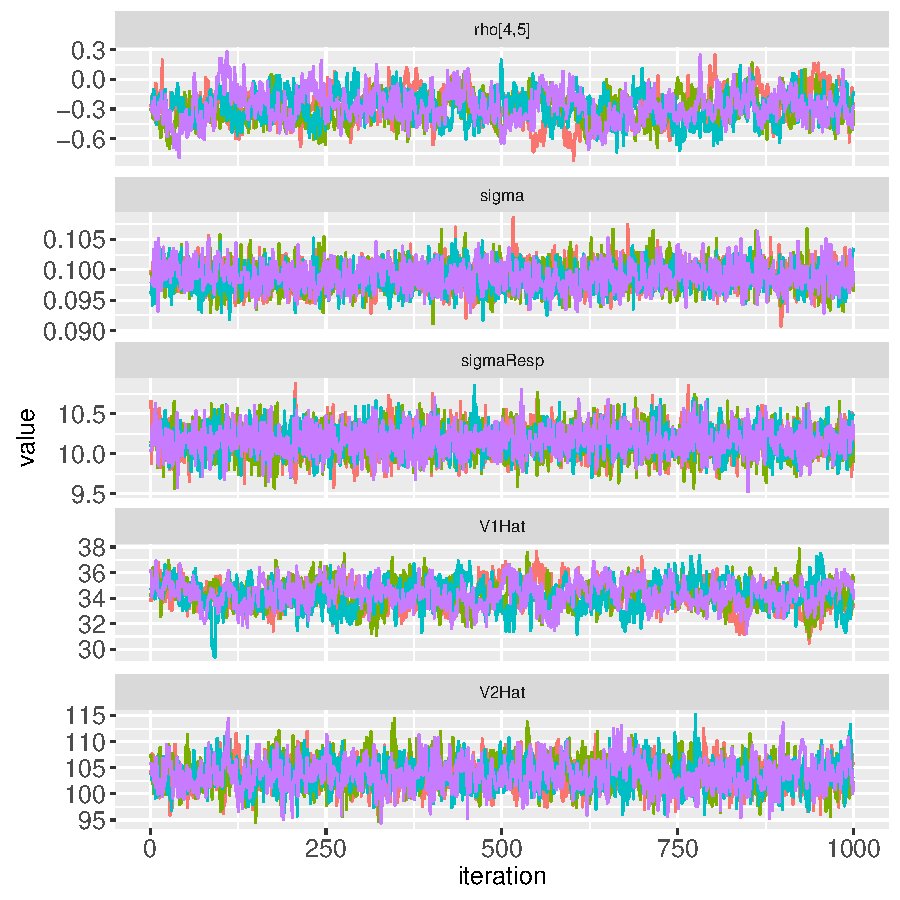
\includegraphics[width=3.0in,trim=0in 0in 0 0in]{graphics/effCptModelTorsten_0.82/effCptPlots005.pdf}
\caption{{MCMC history plots for the parameters of an Effect Compartment Model (each color corresponds to a different chain) for example 2}}
\label{effCptModelMCMC}
\end{figure}

\begin{figure}[!htb]
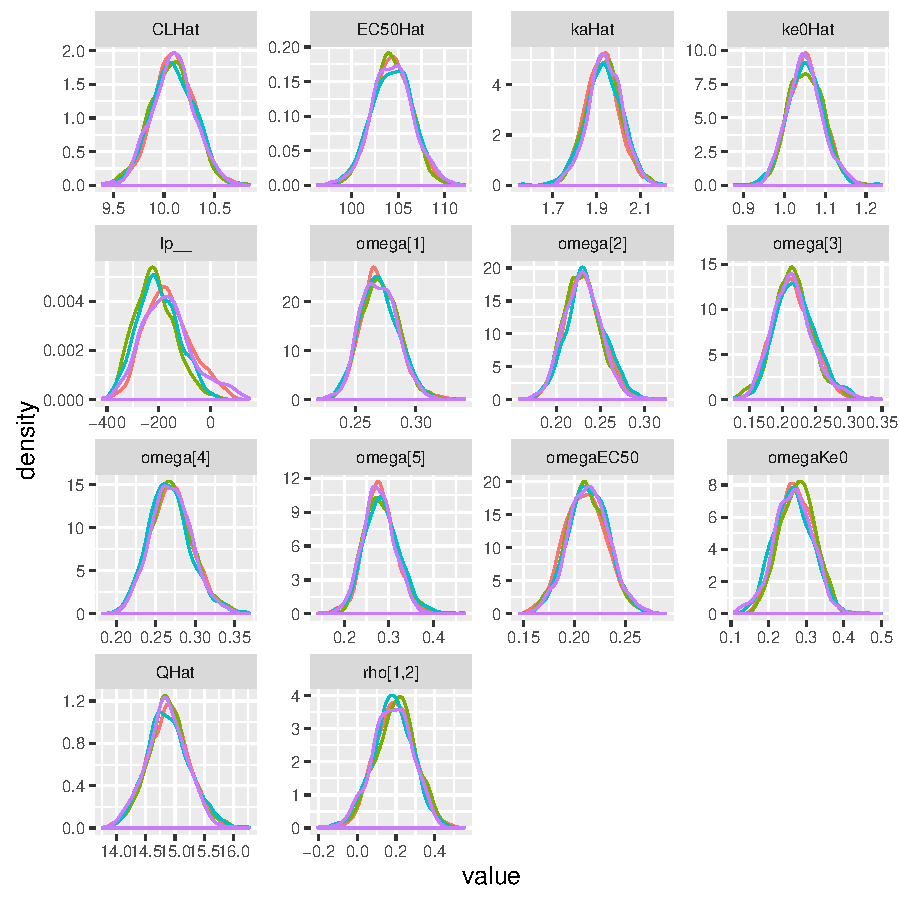
\includegraphics[width=3.0in,trim=0in 0in 0 0in]{graphics/effCptModelTorsten_0.82/effCptPlots006.pdf}
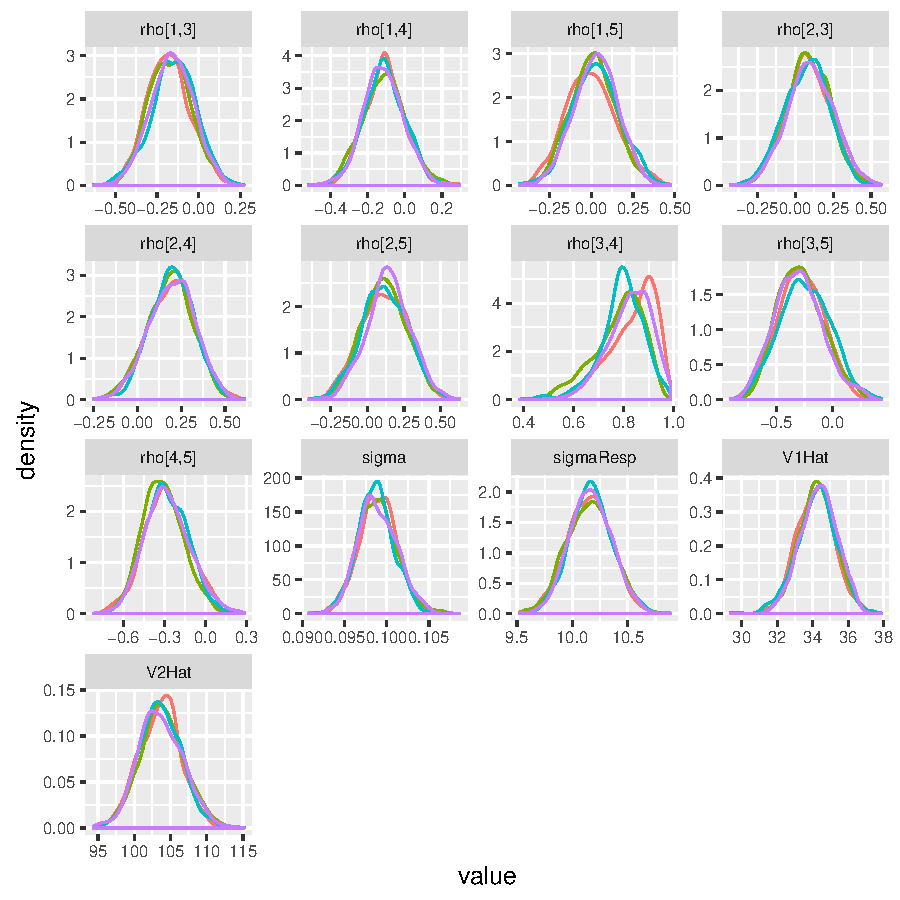
\includegraphics[width=3.0in,trim=0in 0in 0 0in]{graphics/effCptModelTorsten_0.82/effCptPlots007.pdf}
\caption{{Posterior Marginal Densities of the Model Parameters of an Effect Compartment Model (each color corresponds to a different chain) for example 2}}
\label{effCptModelDens}
\end{figure}

\begin{figure}[htbp]
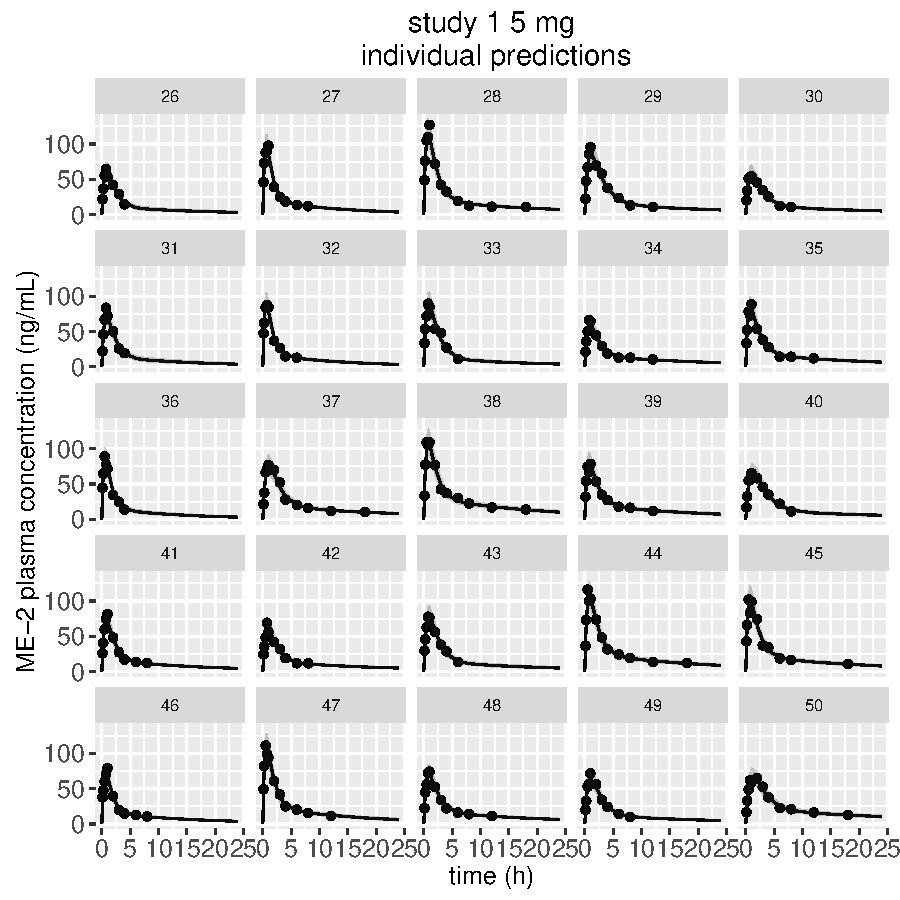
\includegraphics[width=1.5in,trim=0in 0in 0 0in]{graphics/effCptModelTorsten_0.82/effCptPlots011.pdf}
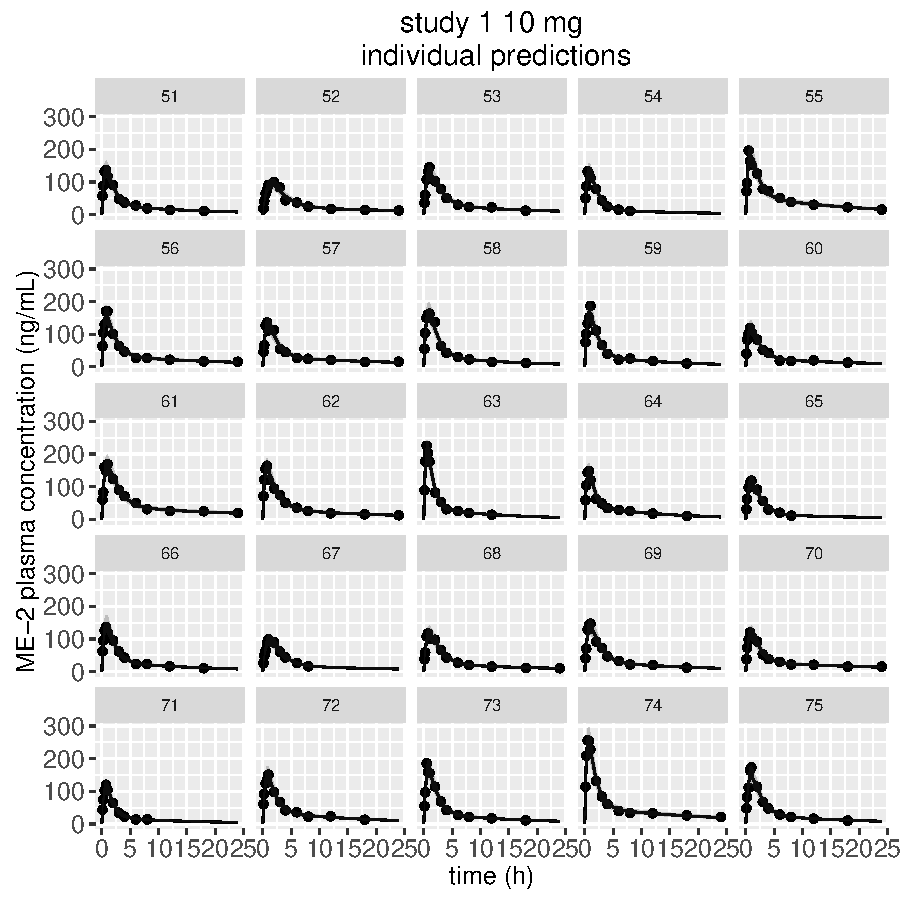
\includegraphics[width=1.5in,trim=0in 0in 0 0in]{graphics/effCptModelTorsten_0.82/effCptPlots012.pdf}
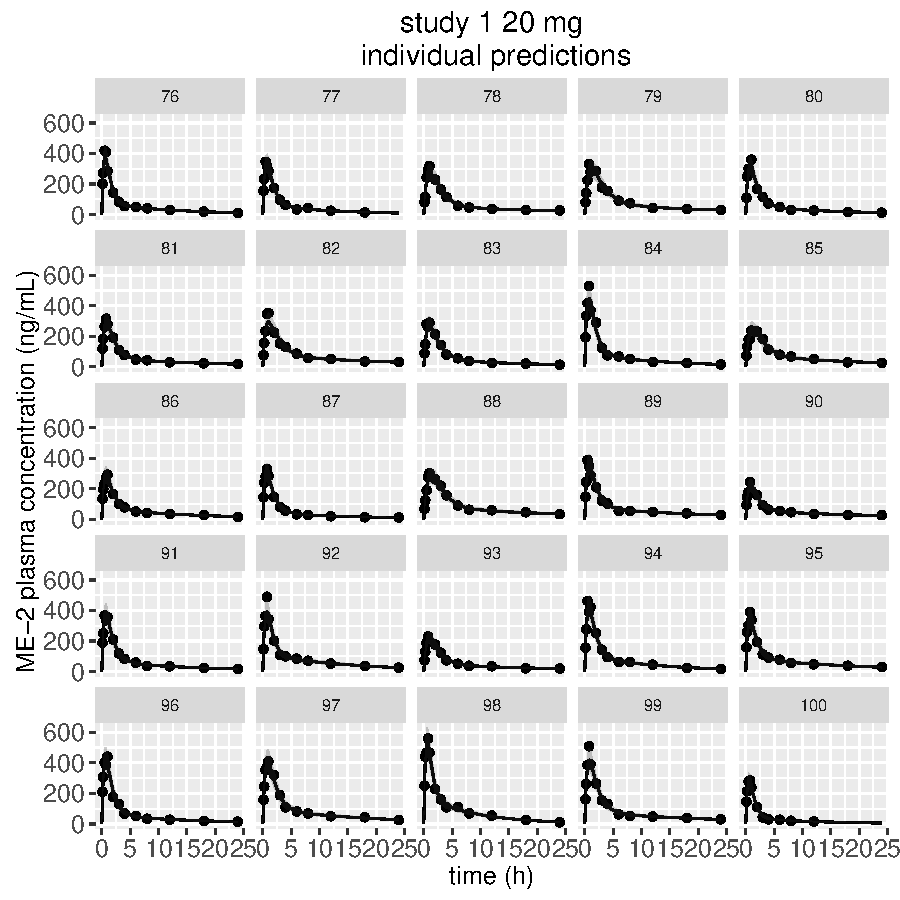
\includegraphics[width=1.5in,trim=0in 0in 0 0in]{graphics/effCptModelTorsten_0.82/effCptPlots013.pdf}
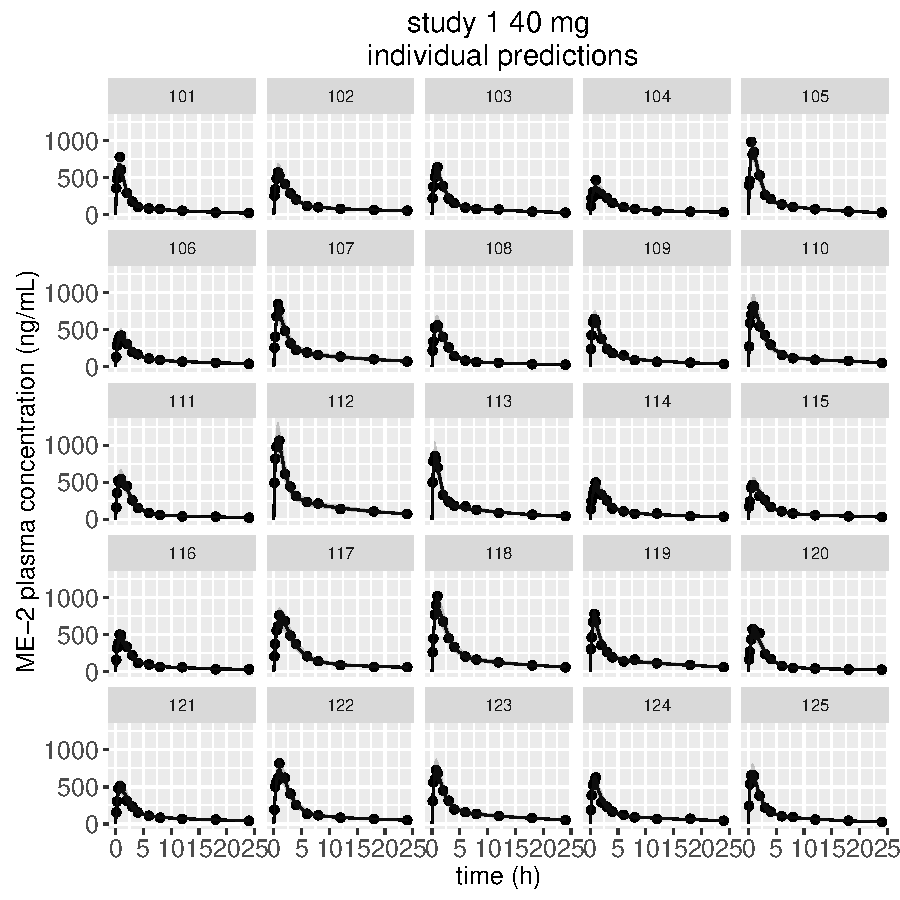
\includegraphics[width=1.5in,trim=0in 0in 0 0in]{graphics/effCptModelTorsten_0.82/effCptPlots014.pdf}
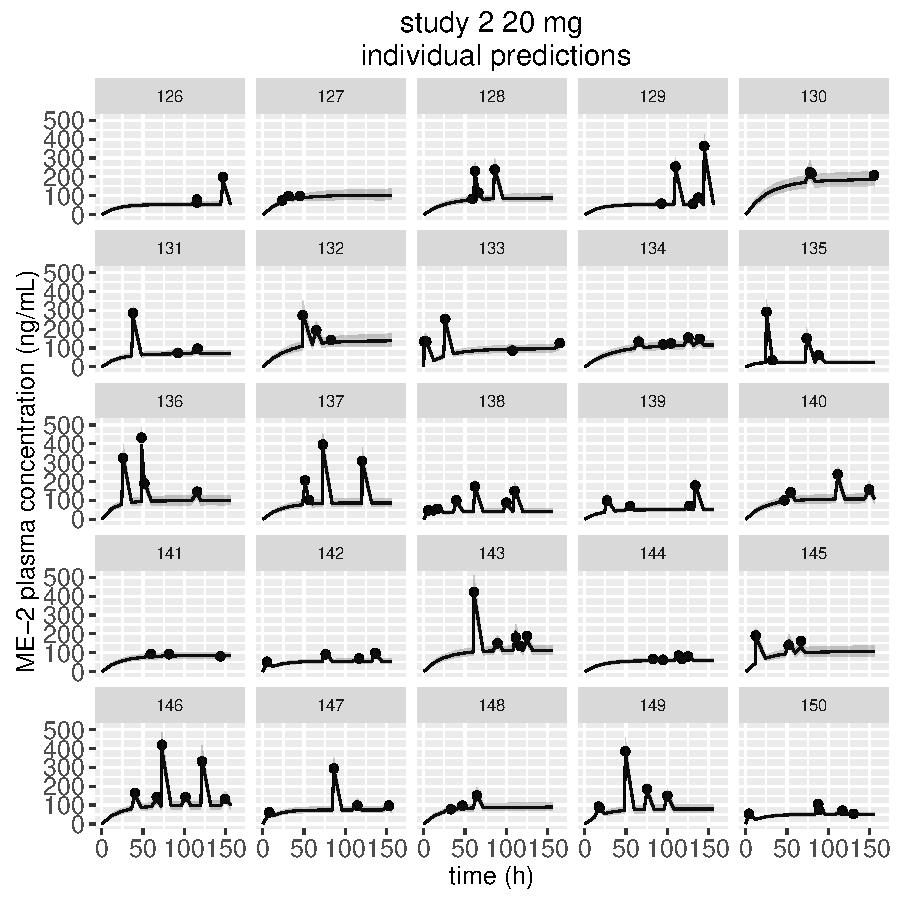
\includegraphics[width=1.5in,trim=0in 0in 0 0in]{graphics/effCptModelTorsten_0.82/effCptPlots019.pdf}
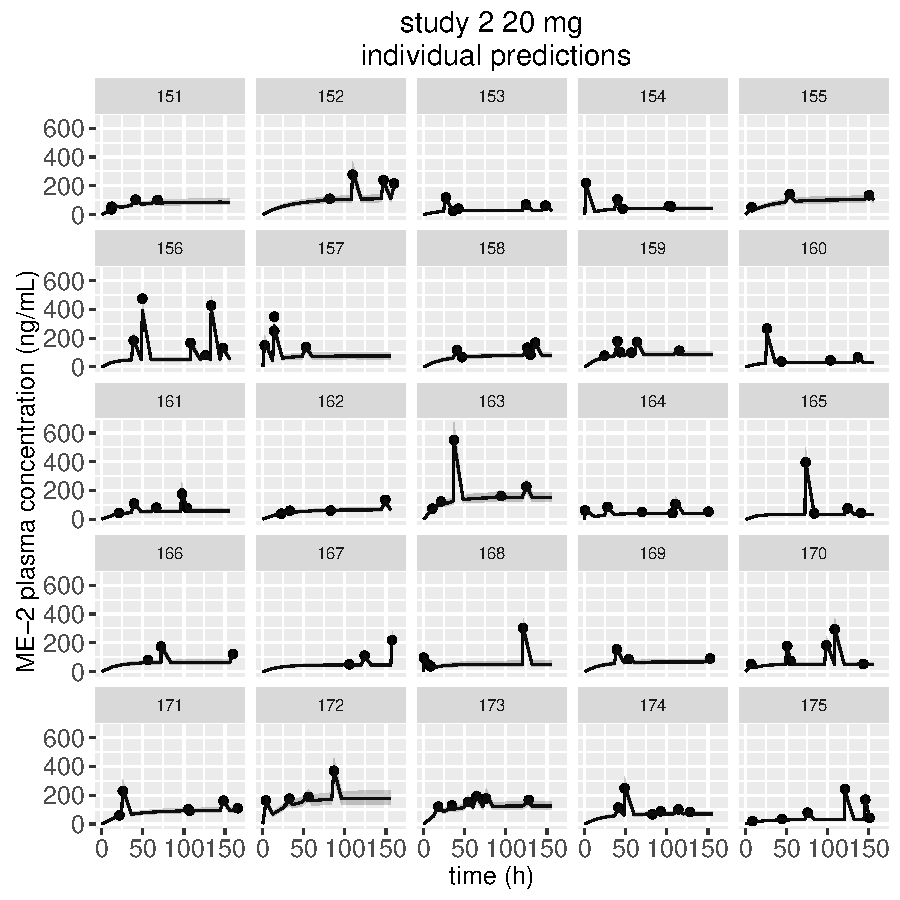
\includegraphics[width=1.5in,trim=0in 0in 0 0in]{graphics/effCptModelTorsten_0.82/effCptPlots020.pdf}
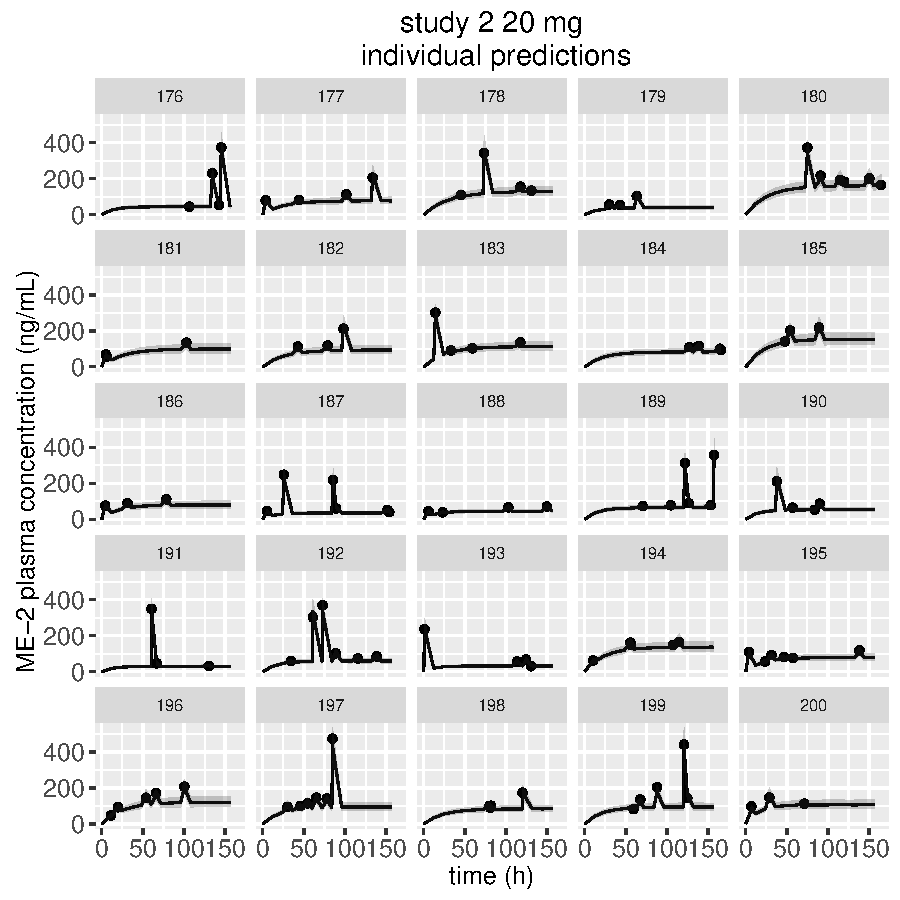
\includegraphics[width=1.5in,trim=0in 0in 0 0in]{graphics/effCptModelTorsten_0.82/effCptPlots021.pdf}
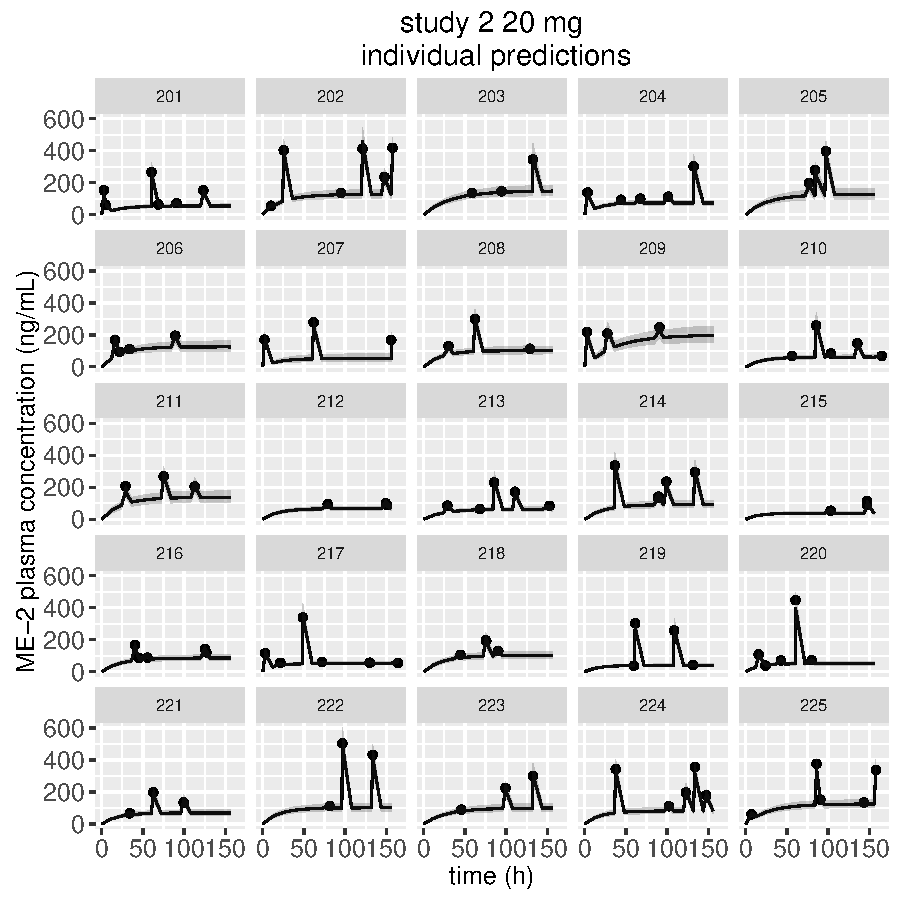
\includegraphics[width=1.5in,trim=0in 0in 0 0in]{graphics/effCptModelTorsten_0.82/effCptPlots022.pdf}
\caption{{Predicted (posterior median and 90 \% credible intervals) and observed plasma drug concentrations for example 2 for an Effect Compartment Model}}
\label{effCptModelPredictionsPK}
\end{figure}

\begin{figure}[htbp]
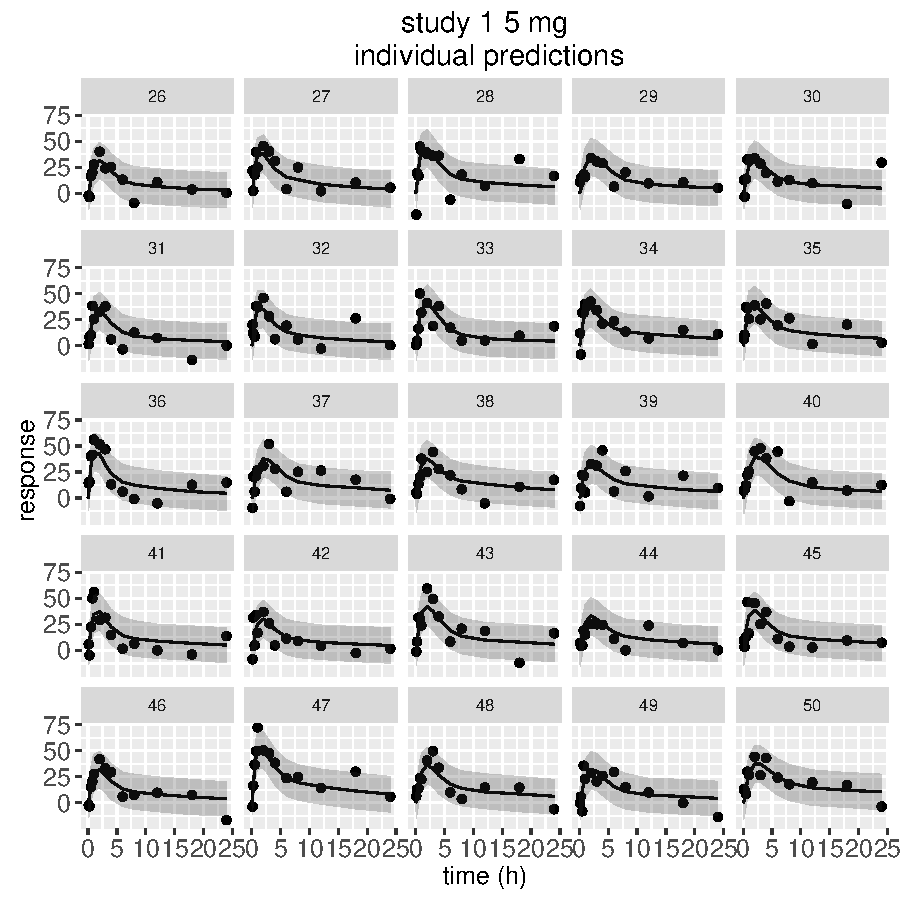
\includegraphics[width=1.5in,trim=0in 0in 0 0in]{graphics/effCptModelTorsten_0.82/effCptPlots023.pdf}
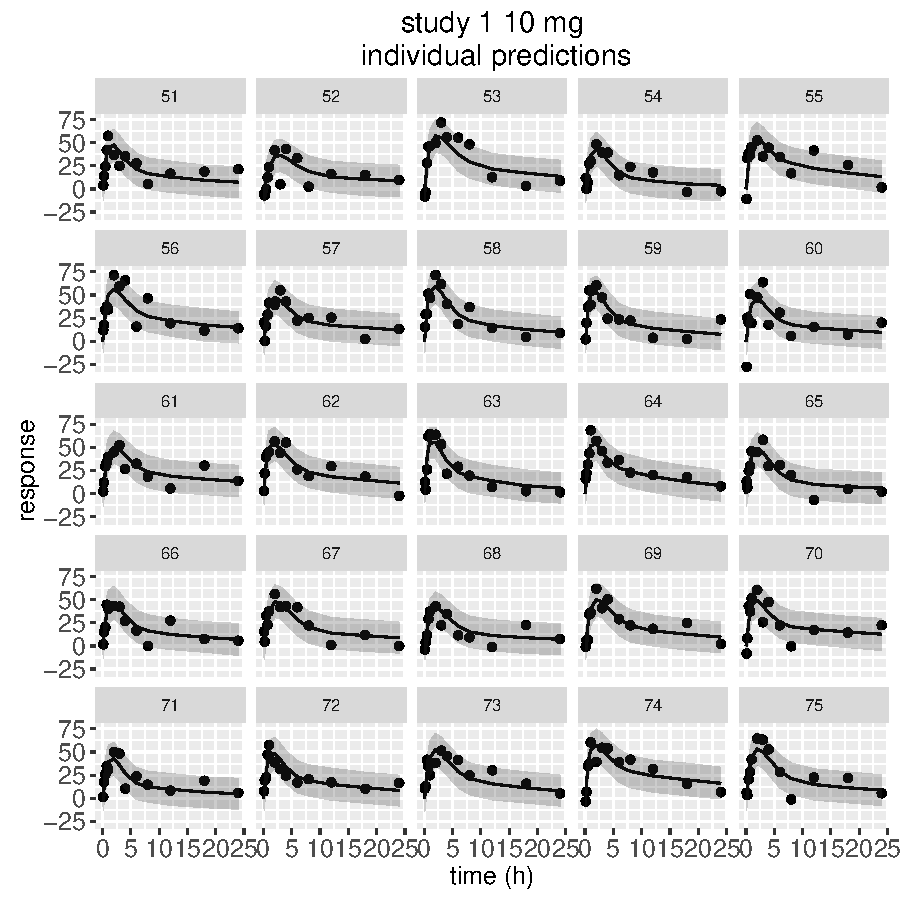
\includegraphics[width=1.5in,trim=0in 0in 0 0in]{graphics/effCptModelTorsten_0.82/effCptPlots024.pdf}
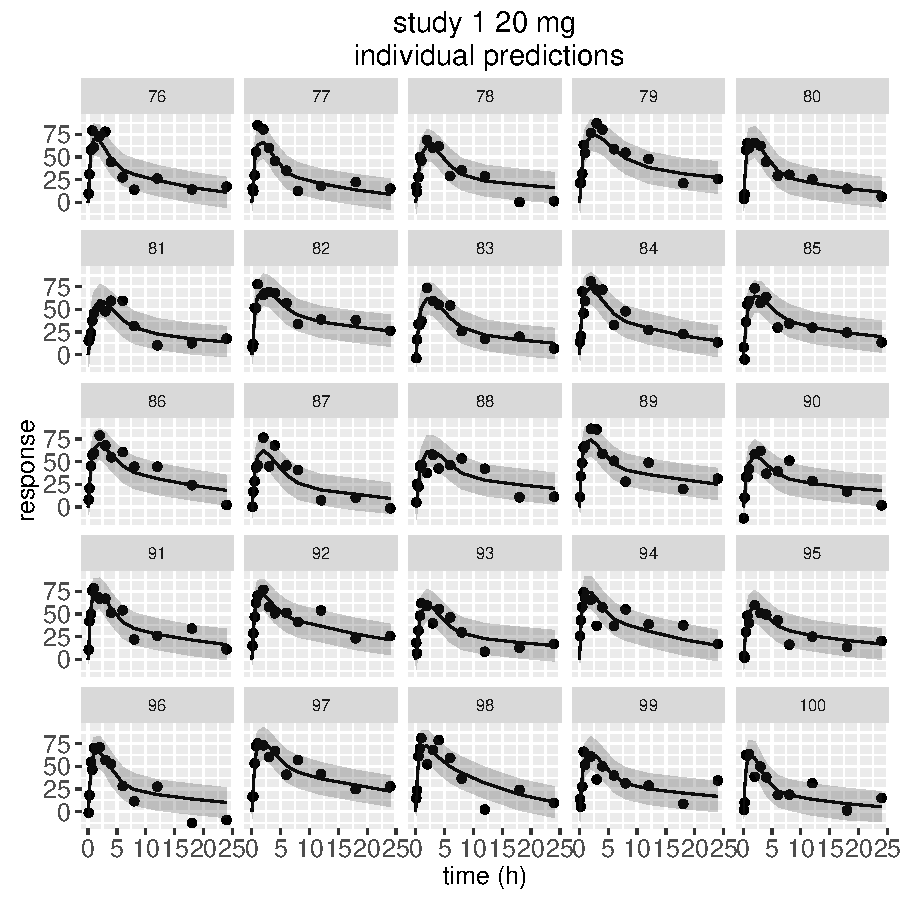
\includegraphics[width=1.5in,trim=0in 0in 0 0in]{graphics/effCptModelTorsten_0.82/effCptPlots025.pdf}
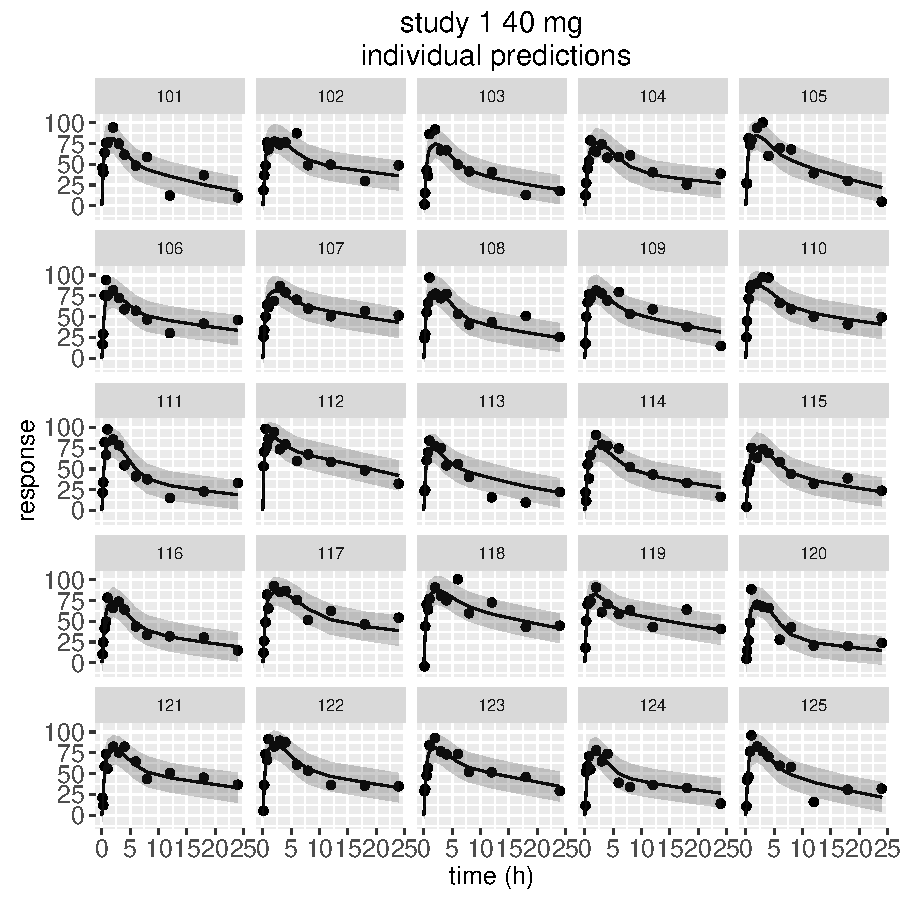
\includegraphics[width=1.5in,trim=0in 0in 0 0in]{graphics/effCptModelTorsten_0.82/effCptPlots026.pdf}
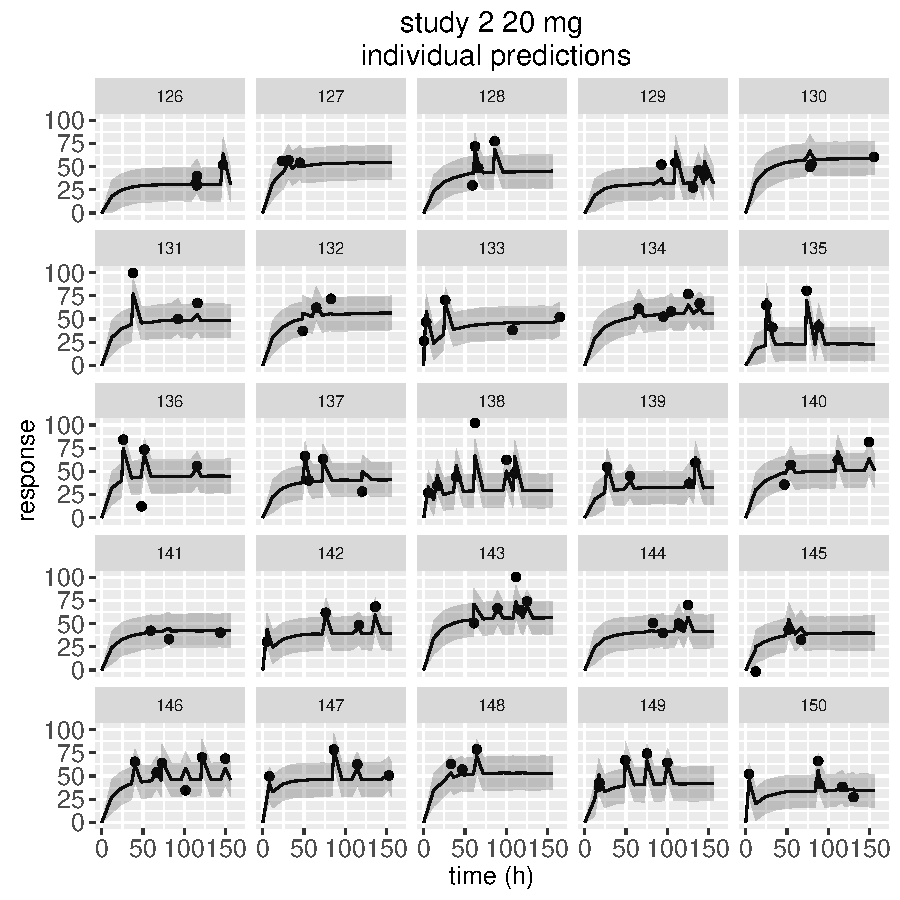
\includegraphics[width=1.5in,trim=0in 0in 0 0in]{graphics/effCptModelTorsten_0.82/effCptPlots027.pdf}
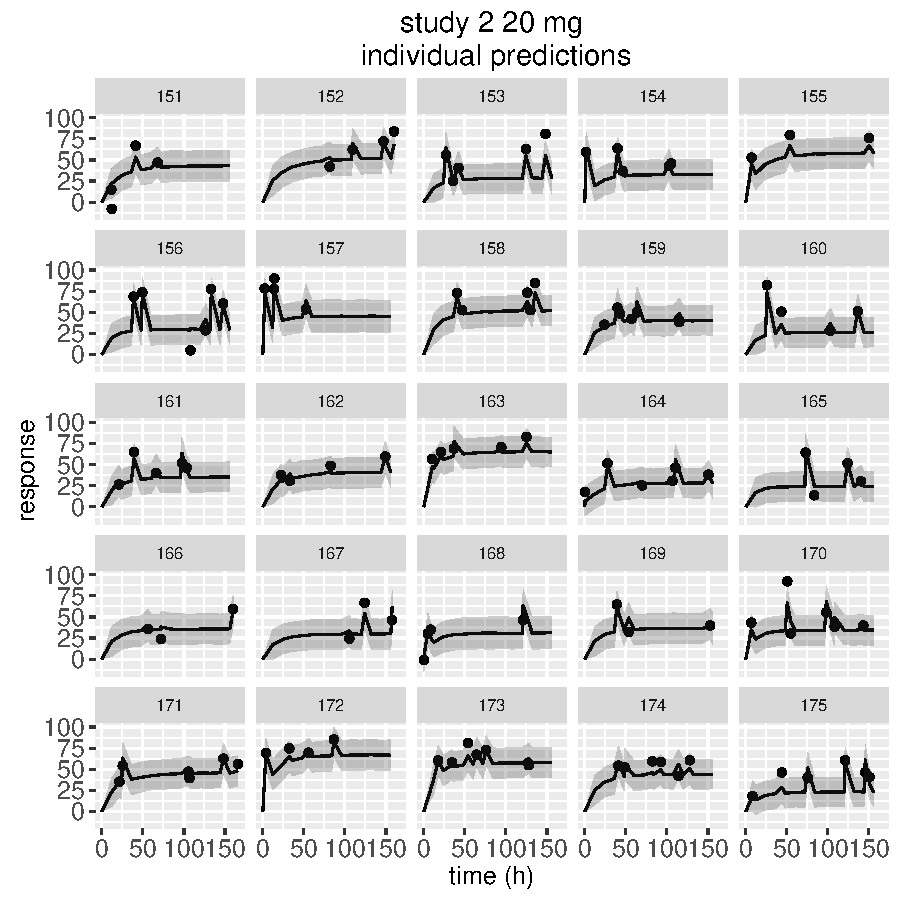
\includegraphics[width=1.5in,trim=0in 0in 0 0in]{graphics/effCptModelTorsten_0.82/effCptPlots028.pdf}
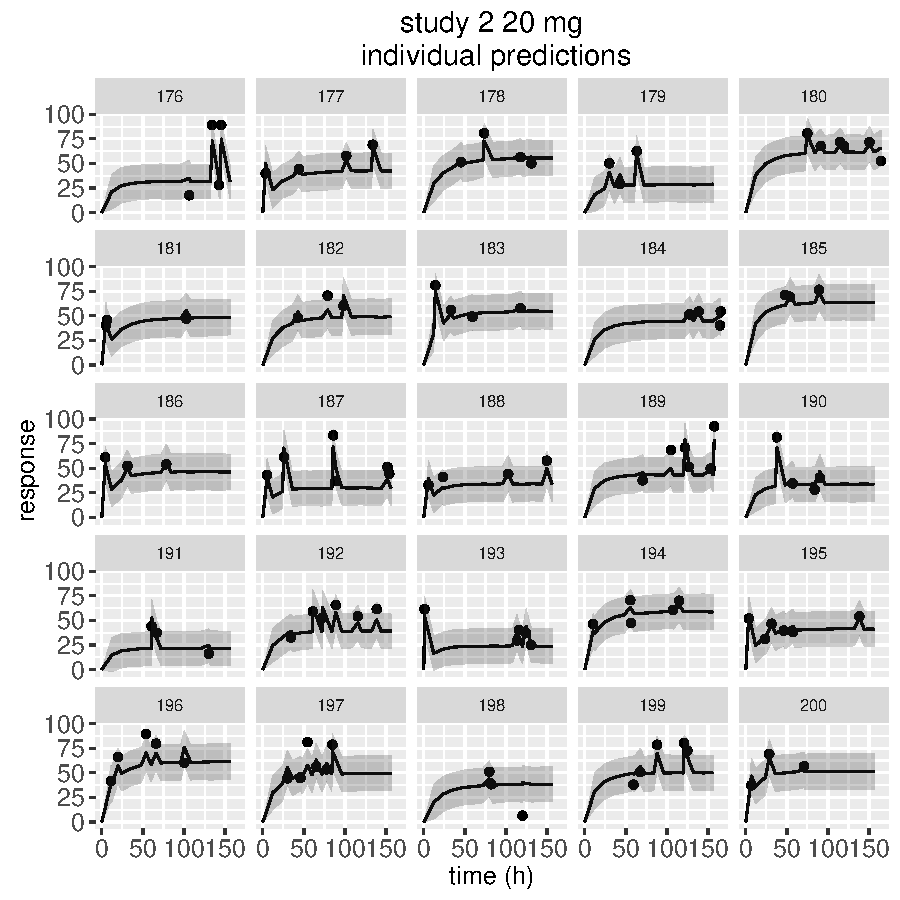
\includegraphics[width=1.5in,trim=0in 0in 0 0in]{graphics/effCptModelTorsten_0.82/effCptPlots029.pdf}
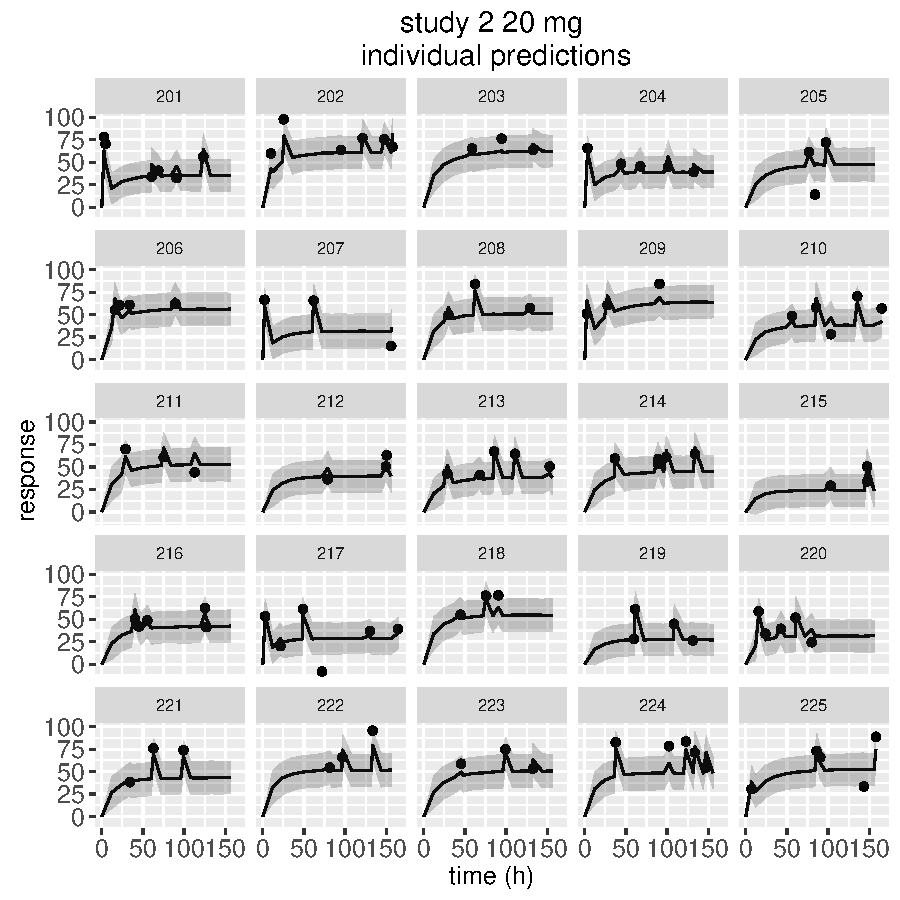
\includegraphics[width=1.5in,trim=0in 0in 0 0in]{graphics/effCptModelTorsten_0.82/effCptPlots030.pdf}
\caption{{Predicted (posterior median and 90 \% credible intervals) and observed PD Response for example 2}}
\label{effCptModelPredictionsPD}
\end{figure}

\clearpage

\subsection{Example 4: Friberg-Karlsson Semi-Mechanistic Population Model} \ \\ 

We now return to example 2 and extend it to a population model. While we recommend using the mixed solver, for completeness we'll show how to specify the model with the \texttt{generalOdeModel\_*} function. We leave it as an exercise to the reader to rewrite the model with \texttt{mixOde2CptModel\_*}. 

{\bf Friberg-Karlsson Population Model for drug-induced myelosuppression ($ANC$)}

\begin{eqnarray*}
\log(ANC_{ij}) &\sim& N(Circ_{ij}, \sigma^2_{ANC}) \\
\log\left(MTT_j, Circ_{0j}, \alpha_j\right) &\sim& N\left(\log\left(\widehat{MTT}, \widehat{Circ_0}, \widehat{\alpha}\right), \Omega_{ANC}\right) \\
\left(\widehat{MTT}, \widehat{Circ}_0,\widehat{\alpha}, \gamma \right) &=& \left(125, 5, 2, 0.17\right) \\
\Omega_{ANC} &=& \left(\begin{array}{ccc} 0.2^2 & 0 & 0 \\ 0 & 0.35^2 & 0 \\ 0 & 0 & 0.2^2 \end{array}\right), \ \ \ \sigma_{ANC} = 0.1 \\
\Omega_{PK} &=& \left(\begin{array}{ccccc} 0.25^2 & 0 &a 0 & 0 & 0 \\ 0 & 0.4^2 & 0 & 0 & 0 \\
0 & 0 & 0.25^2 & 0 & 0 \\ 0 & 0 & 0 & 0.4^2 & 0 \\ 0 & 0 & 0 & 0 & 0.25^2  \end{array}\right)
\end{eqnarray*}

The PK and the PD data are simulated using the following treatment.
\begin{itemize}
  \item Phase IIa trial in patients
  \begin{itemize}
    \item Multiple doses: 80,000 mg
    \item Parallel dose escalation design
    \item 15 subjects
    \item PK: plasma concentration of parent drug ($c$)
    \item PD response: Neutrophil count ($ANC$)
    \item PK measured at 0.083, 0.167, 0.25, 0.5, 0.75, 1, 2, 3, 4, 6, 8, 12, 18, and 24 hours
    \item PD measured once every two days for 28 days.
  \end{itemize}
\end{itemize}

Once again, we simultaneously fit the model to the PK and the PD
data. Note that from a computational perspective, this is a much more
difficult problem than the one we dealt with in the previous
example. The nonlinear nature of the ODEs forces us to use a numerical
solver, which is significantly slower than the linear methods we have
employed so far. Because the ODE system of interest is non-stiff, we
use the \textit{rk45} version of \texttt{genOdeModel} (Figures
\ref{FKODECode} and \ref{FKCode}).

It pays off to construct informative priors. For instance, we could
fit the PK data first, as was done in  example 1, and get informative
priors on the PK parameters. The PD parameters are drug independent,
so we can use information from the neutropenia literature. In this
example, we choose to use weakly informative priors on the PK
parameters and strongly informative priors on the PD parameters. 

Since it takes a long time to run the model, we only use 100
iterations per chain, and study what we can learn from this less than
optimal scenario. It is worth noting that Stan, because of its highly
efficient MCMC sampler, still does a reasonable job estimating the
posterior distribution.

\begin{figure}
\caption{Stan language for coding an ODE system describing a Friberg-Karlsson Mechanism}
\begin{tiny}
\begin{center}
\begin{fmpage}{\textwidth - .75in}
\begin{lstlisting}[basicstyle=\tiny\ttfamily,mathescape=true,flexiblecolumns=true,frame=single,escapeinside=`']
    real[] twoCptNeutModelODE(real t,
			real[] x,
			real[] parms,
			real[] rdummy,
			int[] idummy){
    real CL = parms[1];
    real Q = parms[2];
    real V2 = parms[3];
    real V3 = parms[4];
    real ka = parms[5];
    real mtt = parms[6];
    real circ0 = parms[7];
    real gamma = parms[8];
    real alpha = parns[9];
    real k10 = CL / V2;
    real k12 = Q / V2;
    real k21 = Q / V3;
    real ktr = 4 / mtt;
    real dxdt[8];
    real conc;
    real EDrug;
    real transit1;
    real transit2;
    real transit3;
    real circ;
    real prol;
  
    dxdt[1] = -ka * x[1];
    dxdt[2] = ka * x[1] - (k10 + k12) * x[2] + k21 * x[3];
    dxdt[3] = k12 * x[2] - k21 * x[3];
    conc = x[2]/V1;
    EDrug = alpha * conc;
    // x[4], x[5], x[6], x[7] and x[8] are differences from circ0.
    prol = x[4] + circ0;
    transit1 = x[5] + circ0;
    transit2 = x[6] + circ0;
    transit3 = x[7] + circ0;
    circ = fmax(machine_precision(), x[8] + circ0); // Device for implementing a modeled 
                                                                              // initial condition
    dxdt[4] = ktr * prol * ((1 - EDrug) * ((circ0 / circ)^gamma) - 1);
    dxdt[5] = ktr * (prol - transit1);
    dxdt[6] = ktr * (transit1 - transit2);
    dxdt[7] = ktr * (transit2 - transit3);
    dxdt[8] = ktr * (transit3 - circ);

    return dxdt;
  }
\end{lstlisting}
\end{fmpage}
\end{center}
\end{tiny} 
\label{FKODECode}
\end{figure}

\begin{figure}
\caption{Stan language for fitting a Friberg-Karlsson model using \texttt{genCptModel\_rk45} (abstract)}
\begin{tiny}
\begin{center}
\begin{fmpage}{\textwidth - .75in}
\begin{lstlisting}[basicstyle=\tiny\ttfamily,mathescape=true,flexiblecolumns=true,frame=single,escapeinside=`']
transformed parameters {
                             $\vdots$
  for(i in 1:nSubjects) {

    parms[1] = thetaM[i, 1] * (weight[i] / 70)^0.75; # CL
    parms[2] = thetaM[i, 2] * (weight[i] / 70)^0.75; # Q
    parms[3] = thetaM[i, 3] * (weight[i] / 70); # V1
    parms[4] = thetaM[i, 4] * (weight[i] / 70); # V2
    parms[5] = kaHat; # ka
    parms[6] = thetaM[i, 5]; # mtt
    parms[7] = thetaM[i, 6]; # circ0
    parms[8] = gamma;
    parms[9] = thetaM[i, 7]; # alpha

    x[start[i]:end[i]] = `\textcolor{red}{generalOdeModel\_rk45}'(twoCptNeutModelODE, 8,
                                                           time[start[i]:end[i]], 
                                                           amt[start[i]:end[i]], 
                                                           rate[start[i]:end[i]], 
                                                           ii[start[i]:end[i]], 
                                                           evid[start[i]:end[i]], 
                                                           cmt[start[i]:end[i]], 
                                                           addl[start[i]:end[i]], 
                                                           ss[start[i]:end[i]],
                                                           parms, F, tlag,
                                                           1e-6, 1e-6, 1e6);

    cHat[start[i]:end[i]] = x[start[i]:end[i], 2] / parms[1][3]; # divide by V1
    neutHat[start[i]:end[i]] = x[start[i]:end[i], 8] + parms[1][7]; # Add baseline
    
  }
  
  cHatObs = cHat[iObsPK];
  neutHatObs = neutHat[iObsPD];

                             $\vdots$  
\end{lstlisting}
\end{fmpage}
\end{center}
\end{tiny} 
\label{FKCode}
\end{figure}

\subsubsection*{Results} The MCMC history plots are not as convincing
as in the previous examples, mostly because the number of iterations
is small (100 versus 1000 in the previous example) (Figure
\ref{FKMCMC}. It does however look as though the chains are converging
to a common distribution, and we see little auto-correlation (in
particular, we expect that if we had run the model for 1000
iterations, we would obtain the desired ``fuzzy caterpillar"
look). The model fits the data, and the credible interval reflect the
noise in the data (Figure \ref{FKPredictions}). The parameters
estimation reflects the real value of the parameters (Table
\ref{FKParms} and Figure \ref{FKDens}).

{\tiny
\begin{table}[!htb]
\centering
\caption{Summary of the MCMC simulations of the marginal posterior
  distributions of the model parameters for the Friberg-Karlsson model
example.}
\label{FKParms}
\begin{tabular}{rrrrrrrrrrr}
  \hline
 & mean & se\_mean & sd & 2.5\% & 25\% & 50\% & 75\% & 97.5\% & n\_eff & Rhat \\ 
  \hline
CL & 9.986 & 0.009 & 0.174 & 9.641 & 9.872 & 9.982 & 10.107 & 10.331 & 400.000 & 0.997 \\
Q & 14.633 & 0.055 & 1.106 & 12.505 & 13.992 & 14.623 & 15.296 & 16.948 & 400.000 & 0.996 \\
V1 & 32.909 & 0.174 & 2.439 & 28.203 & 31.186 & 32.836 & 34.762 & 37.750 & 195.828 & 1.008 \\
V2 & 106.631 & 0.311 & 6.226 & 95.234 & 102.269 & 106.403 & 111.000 & 118.533 & 400.000 & 0.999 \\
ka & 1.882 & 0.012 & 0.175 & 1.582 & 1.756 & 1.871 & 2.006 & 2.223 & 196.052 & 1.007 \\
sigma & 0.106 & 0.001 & 0.010 & 0.089 & 0.098 & 0.105 & 0.112 & 0.132 & 259.693 & 1.009 \\
alpha & 3.3E-04 & 1.4E-06 & 2.2E-05 & 2.9E-04 & 3.2E-04 & 3.3E-04 & 3.5E-04 & 3.8E-04 & 247 & 1.01 \\
mtt & 132.763 & 0.515 & 6.498 & 120.843 & 128.082 & 132.223 & 136.694 & 146.845 & 159.372 & 1.024 \\
circ0 & 5.014 & 0.009 & 0.172 & 4.711 & 4.888 & 5.000 & 5.138 & 5.334 & 400.000 & 1.000 \\
gamma & 0.190 & 0.002 & 0.022 & 0.153 & 0.175 & 0.187 & 0.202 & 0.239 & 139.485 & 1.025 \\
sigmaNeut & 0.092 & 0.001 & 0.014 & 0.068 & 0.082 & 0.090 & 0.100 & 0.125 & 161.199 & 1.010 \\
  \hline
\end{tabular}
\end{table} 
}

\begin{figure}[htbp]
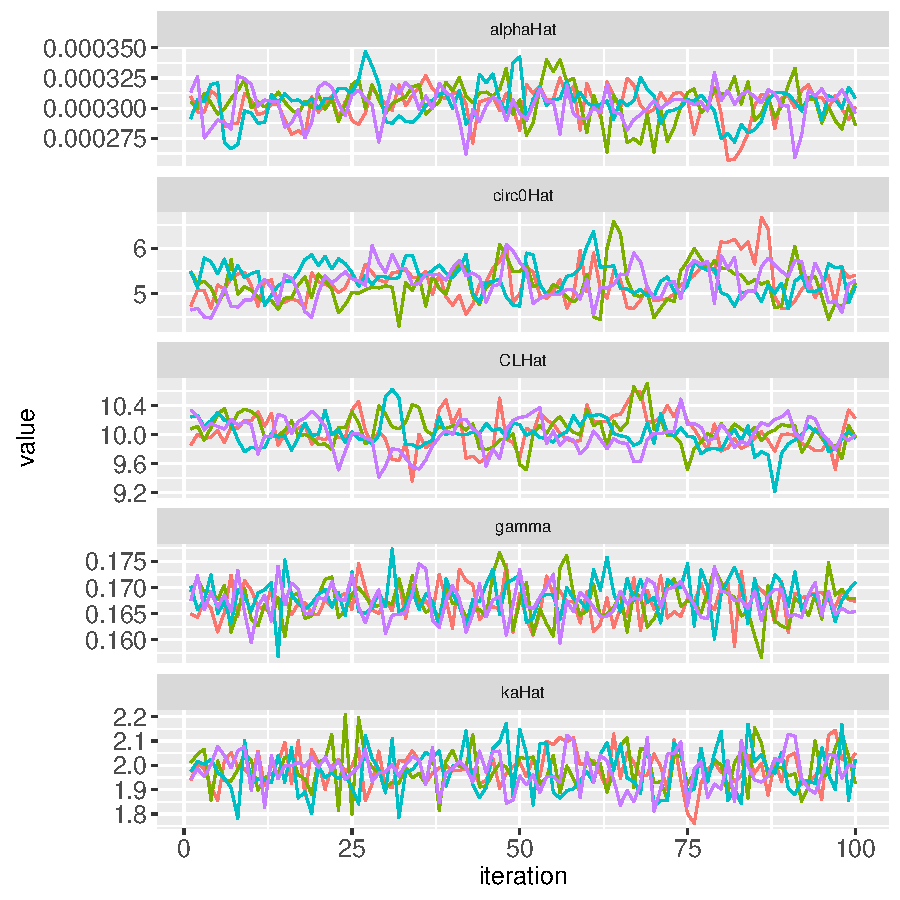
\includegraphics[width=3.0in,trim=0in 0in 0 0in]{graphics/neutropenia_0.82/neutropeniaPopulationPlots001.pdf}
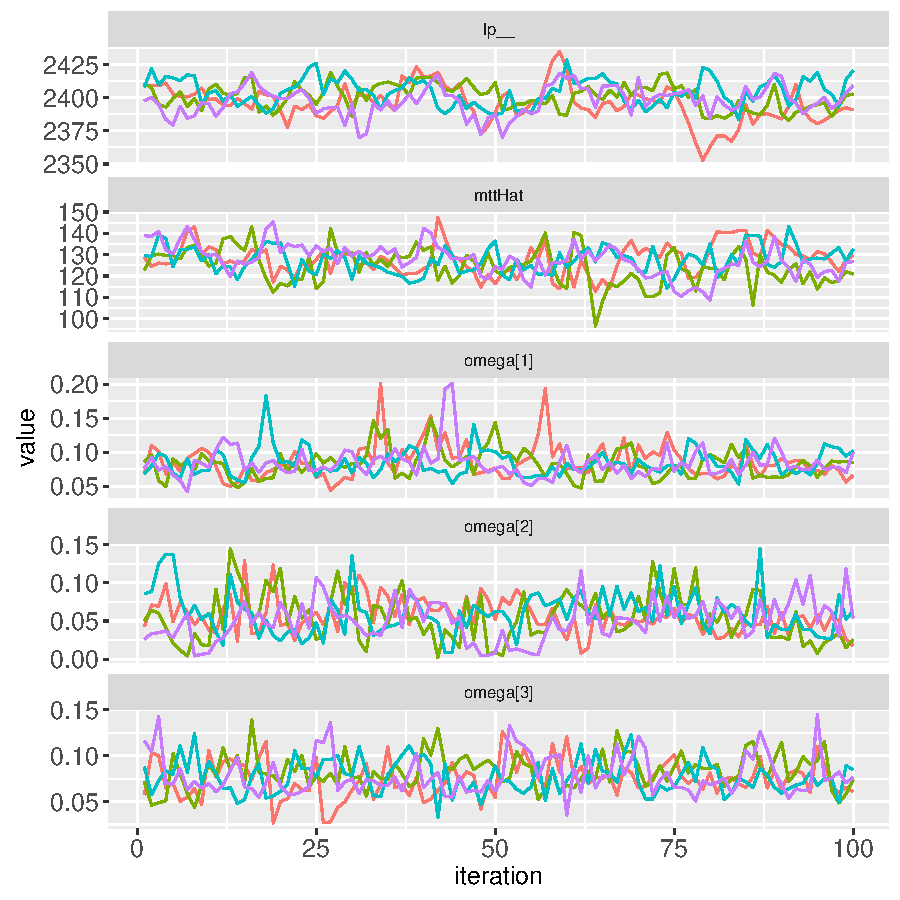
\includegraphics[width=3.0in,trim=0in 0in 0 0in]{graphics/neutropenia_0.82/neutropeniaPopulationPlots002.pdf}
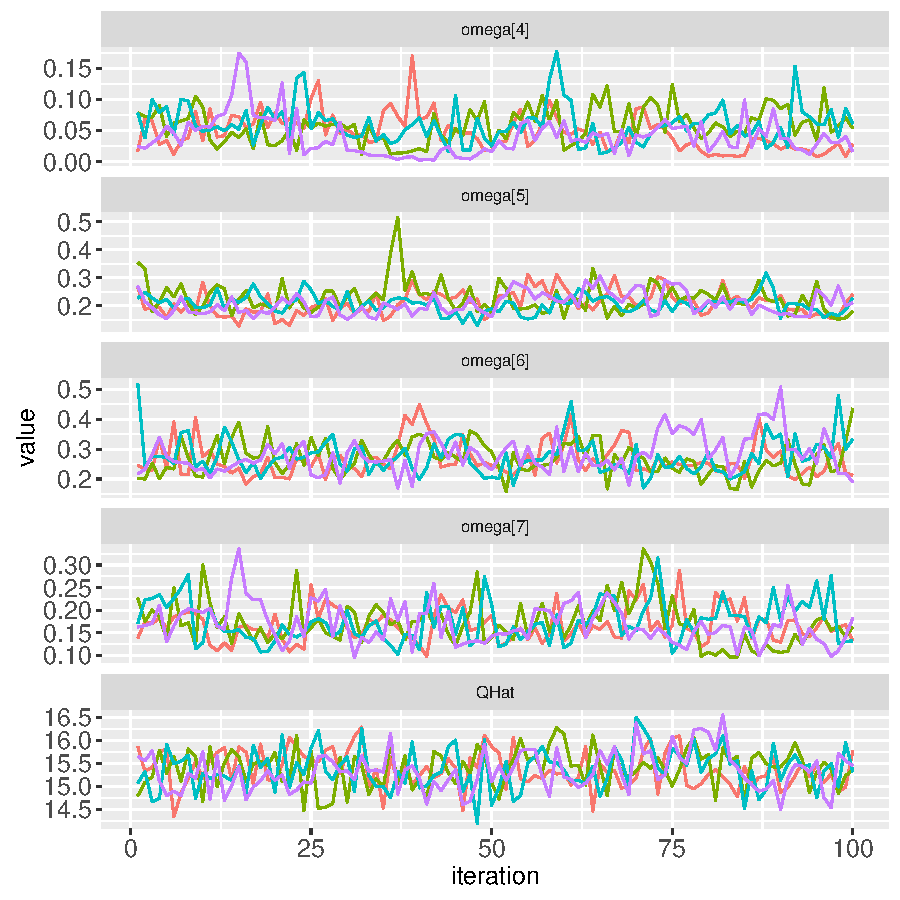
\includegraphics[width=3.0in,trim=0in 0in 0 0in]{graphics/neutropenia_0.82/neutropeniaPopulationPlots003.pdf}
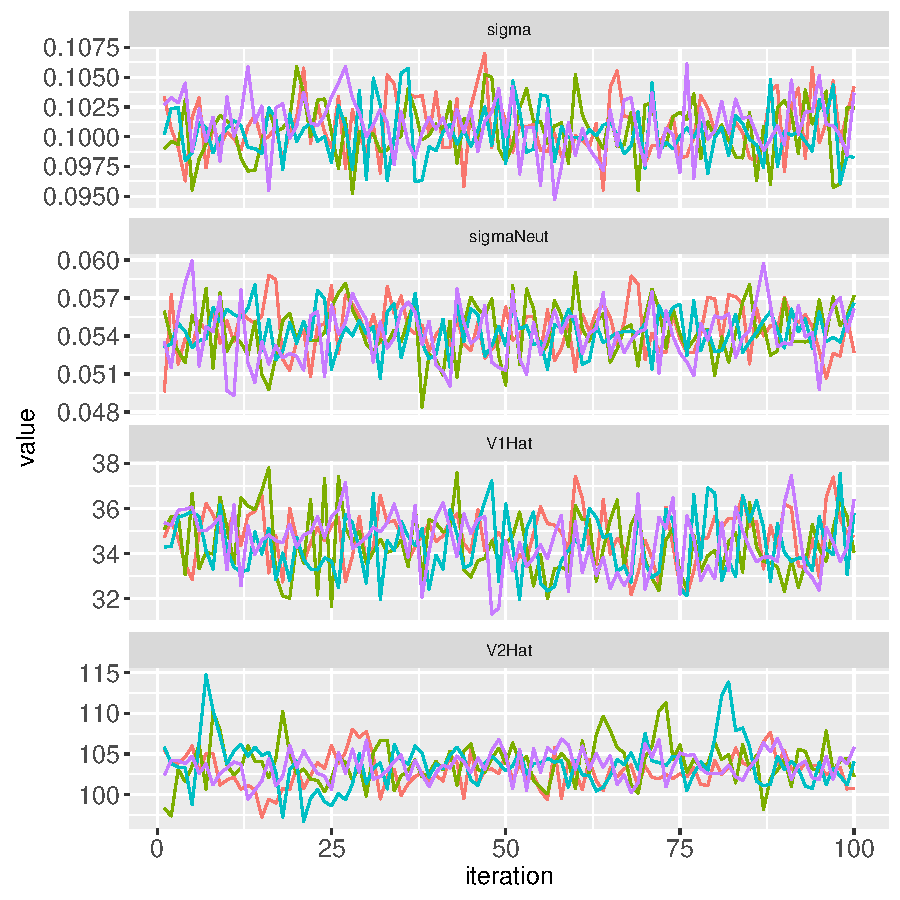
\includegraphics[width=3.0in,trim=0in 0in 0 0in]{graphics/neutropenia_0.82/neutropeniaPopulationPlots004.pdf}
\caption{{MCMC history plots for the parameters of a Friberg-Karlsson semi-mechanistic model (each color corresponds to a different chain) for example 3}}
\label{FKMCMC}
\end{figure}

\begin{figure}[htbp]
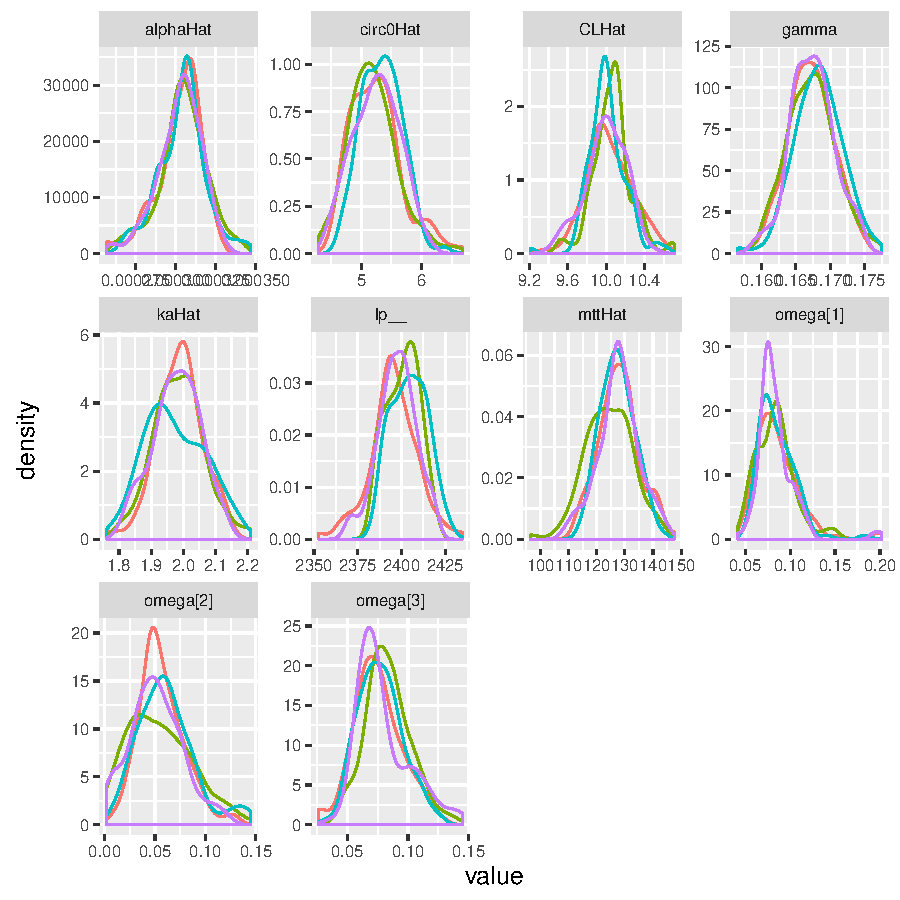
\includegraphics[width=2.5in,trim=0in 0in 0 0in]{graphics/neutropenia_0.82/neutropeniaPopulationPlots005.pdf}
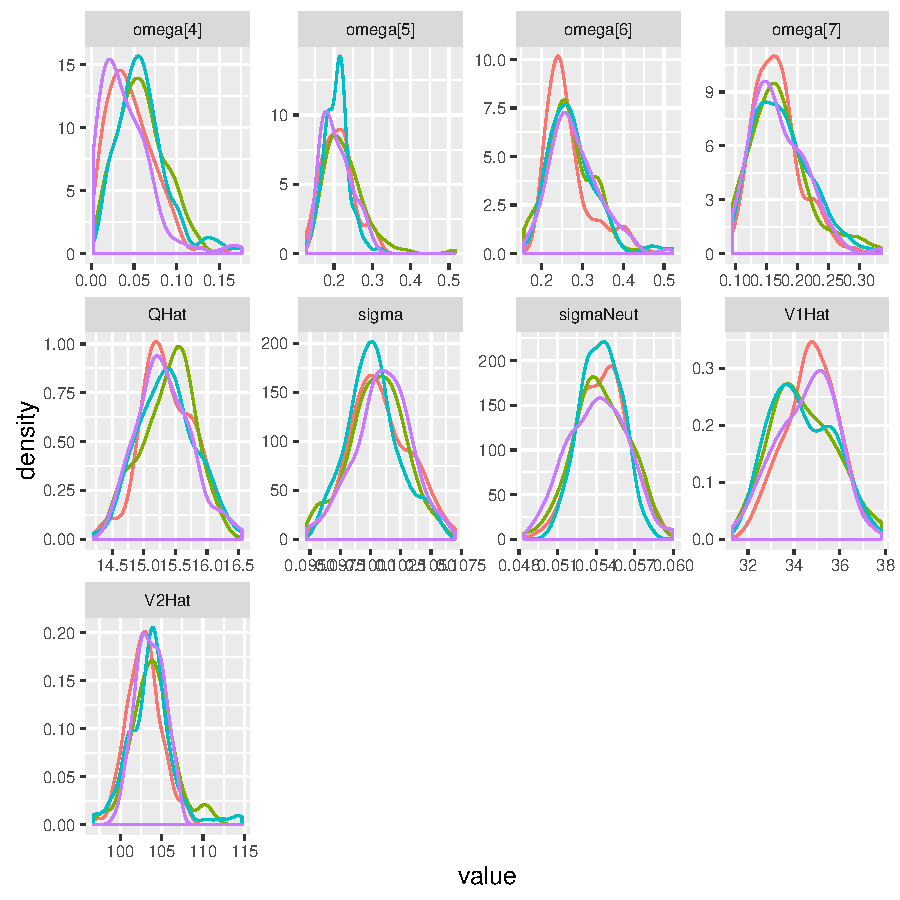
\includegraphics[width=2.5in,trim=0in 0in 0 0in]{graphics/neutropenia_0.82/neutropeniaPopulationPlots006.pdf}
\caption{{Posterior Marginal Densities of the Model Parameters of a Friberg-Karlsson semi-mechanistic model (each color corresponds to a different chain)}}
\label{FKDens}
\end{figure}

\begin{figure}[htbp]
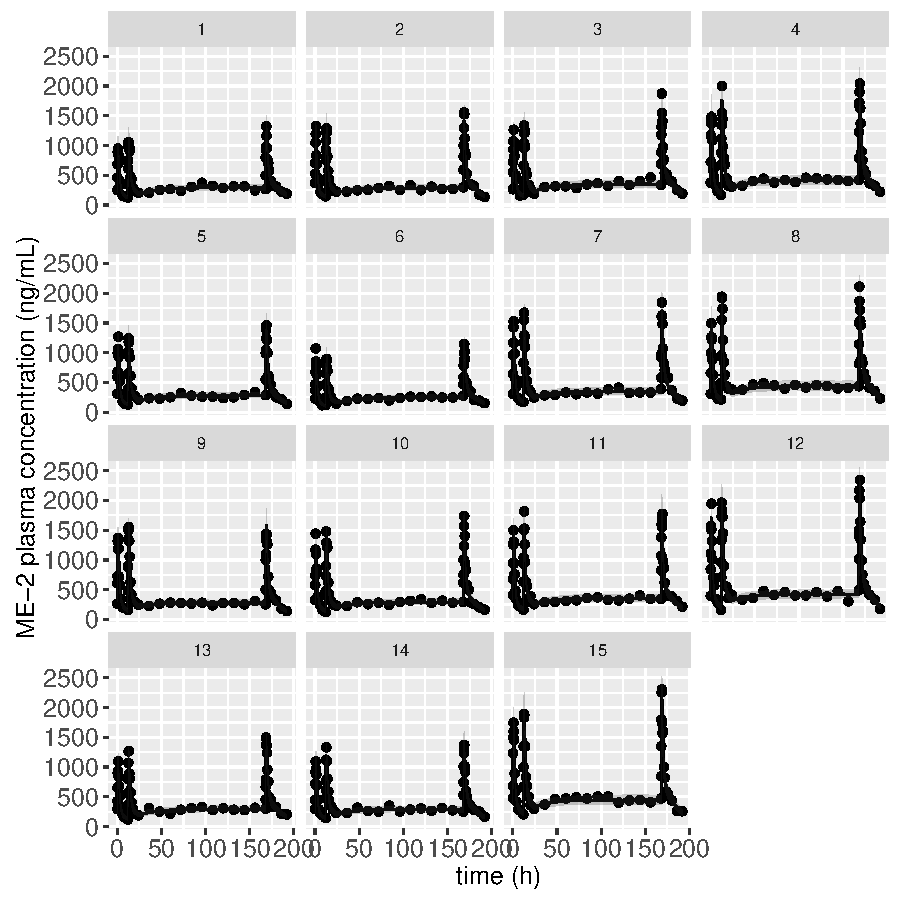
\includegraphics[width=2.5in,trim=0in 0in 0 0in]{graphics/neutropenia_0.82/neutropeniaPopulationPlots010.pdf}
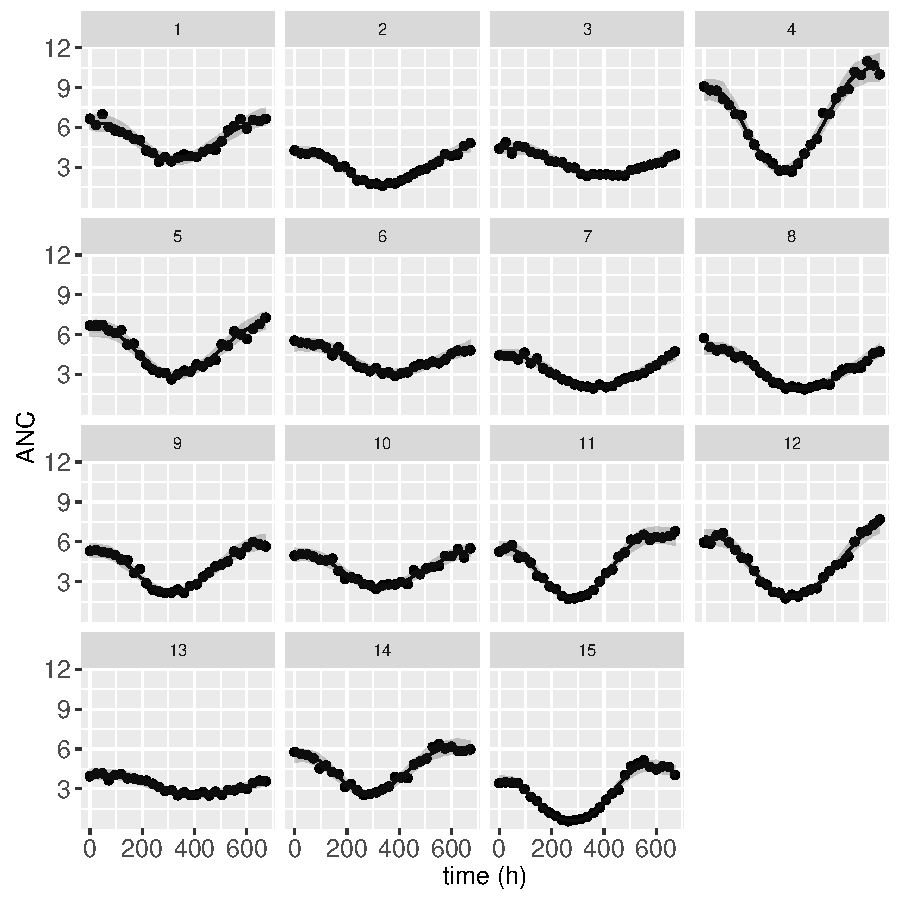
\includegraphics[width=2.5in,trim=0in 0in 0 0in]{graphics/neutropenia_0.82/neutropeniaPopulationPlots011.pdf}
\caption{{Predicted (posterior median and 90 \% credible intervals) and observed plasma drug concentrations, and Neutrophil counts, for a Friberg-Karlsson semi-mechanistic model}}
\label{FKPredictions}
\end{figure}
 
\clearpage

\section{Appendix}

(Note: this section is still being worked on and is far from finished)

%%%%%%%%%%%%%%%%%%%%%%%%%%%%%%%%%%%%%%%%%%%%%%%%%%%%%%%%%%%%%%%%%%%%%%%%
\iffalse

\subsection{Solving Systems of Algebraic Equations} \ \\ \ \\
In order to compute a steady state solution for a general compartment model, we need an algebraic solver. Such a solver will be added to Stan's core language\footnote{A pull request has been submitted on Stan's gitHub page. This prototype builds on the Hybrid Nonlinear solver from the C++ \textit{Eigen} library\cite{eigen}. Their implementation follows closely the one in MINPACK-1\cite{MINPACK}.}. A prototype is available in Torsten's development branch on GitHub.

The \texttt{algebra\_solver} function uses the Powell hybrid method (also called the ``dogleg" method)\cite{dogleg} to find the solution to a system of nonlinear algebraic equations. In other words, we wish to solve:

$$ f(x) = 0 $$

for $x$, where $f$ and $x$ are vector valued functions.

The user first defines $f$, the algebraic system, in the \textbf{functions} block, using a pre-specified signature:

\texttt{real[] f(vector x,  // unknown  \\
\phantom{real[] f} vector y,  // parameters  \\
\phantom{real[] f} real[] dat\_r,  // data (real)  \\
\phantom{real[] f} int[] dat\_int) {  // data (integer)  \\	        
  }  \\
}



The algebraic solver has the form: 

\texttt{algebra\_solver(f,  x, theta,  x\_r, x\_i \\                              
\phantom{algebra\_solver} rel\_tol, f\_tol, max\_step)}

where \texttt{f} is the algebraic system defined in the function block, \texttt{x} a vector which contains the initial guesses for the solution, \texttt{y} a vector of parameters, \texttt{dat\_r} an array of real data, and \texttt{dat\_int} an array of integer data.

The last three arguments are optional and specify the tuning parameters of the solver. The relative tolerance (\texttt{rel\_tol}, default value $1 \times 10^{-10}$) sets an upper bound for the error in the computed solution relative to the real solution. Given an estimated solution $\theta$, the function tolerance (\texttt{f\_tol}, default value $1 \times 10^{-6}$) specifies the maximum value of $||f(\theta)||$\footnote{It helps to think geometrically about this. Ideally we would want the point $f(\theta)$ to be at the origin; the norm represents deviations from this ideal. Users should keep in mind the norm scales up with the square-root of $x$'s dimension.}. The maximum number of steps (\texttt{max\_num\_steps}, default value $1000$) is the maximum number of times the solver will compute $f(x)$ before ``giving up". While these parameters have default values, the user should be prepared to adjust them.

\subsubsection{Example} \ \\ \ \\
Let's suppose we wish to solve the following algebraic system:

\begin{eqnarray*}
  z_1 &=& x_1 - y_1  \\
  z_2 &=& x_2 - y_2
\end{eqnarray*} 

where $(y_1, y_2) = (0.9, 1.1)$. We would code this in Stan as follows:

\begin{figure}[htbp]
\caption{Stan language for solving an algebraic system}
\begin{center}
\begin{small}
\begin{fmpage}{\textwidth - .75in}
\begin{lstlisting}[basicstyle=\footnotesize\ttfamily,mathescape=true,flexiblecolumns=true,frame=single,escapeinside=`']
`\bf{functions}'{
  real[] algebraSystem(vector x,
                              vector y,
                              real[ ] dat,
                              int[ ] dat_int) {	        
    vector[2] f_x;
    f_x[1] = x[1] - y[1];
    f_x[2] = x[2] - y[2];
    return f_x;
  }
}
    $\vdots$

`\bf{transformed data}' {
  vector[2] x;
  vector[2] y;
  real dat[0];
  int dat_int[0];
  
  x[1] = 1;
  x[2] = 1;
}

`\bf{transformed parameters}'{
  vector y[2];
  vector theta[2];
  
  y_p[1] = 0.9;
  y_p[2] = 1.1;
  
  theta = algebra_solver(algebra_system, x, y, dat, dat_int);
}
    $\vdots$
\end{lstlisting}
\end{fmpage}
\end{small}
\end{center}
\label{algebraStan}
\end{figure}


The details we cover here are not required to use Torsten but may be of interest to developers and advanced users. Our goal is to motivate the development of Torsten by looking at common challenges in pharmacometrics. The problems we address are mostly mathematical in nature but scientifically motivated. We discuss why Stan strikes us as a powerful tool to analyse data; and which needs in pharmacometrics Torsten answers. We then go over the algorithms and programming techniques we deploy in Torsten. 

\subsection{Differential Equations Based Models} \ \\ \ \\
The following section is in part based on a presentation we gave at the 2017 Stan Conference \cite{StanCon2017} and motivates the use of Ordinary Differential Equations (ODEs) in pharmacometrics.

\subsubsection{When do Ordinary Differential Equations Arise?} \ \\ \ \\
We deal with an ODE when we want to determine a function $y(t)$ at a specific time but only know the derivative of that function, $\frac{dy}{dt}$. In other words, we know the rate at which a quantity of interest changes but not the quantity itself. In many scenarios, the rate depends on the quantity itself.

\begin{figure}[!htb]
\begin{center}
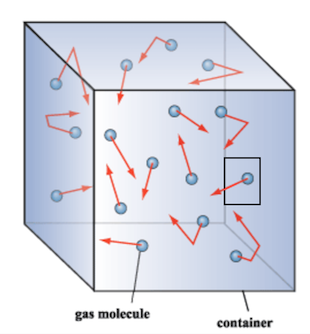
\includegraphics[width=2.0in,trim=0in 0in 0 0in]{graphics/appendix/gas-container.png}
\caption{{Gas container with a hole. The rate at which the gas leaks is proportional to the amount of gas in the container. We can describe this physical process using the differential equation $ \frac{dy}{dt} = -ky(t)$, where $y$ is the amount of gas in the container. \textbf{Will need to create our own figure}}}
\label{GasContainer}
\end{center}
\end{figure}

To get a basic intuition, let us consider an example. Imagine a gas container with a hole in it  (Figure~\ref{GasContainer}). We can think of the gas as being made of molecules that move randomly in the container. Each molecule has a small chance of leaking through the hole. Thus the more molecules inside the container, the higher the number of escaping molecules per unit time. If there are a large number of molecules, and the gas behaves like a continuous fluid, we observe that the more gas in the container, the higher the leakage. This statement can be written as the differential equation:

$$ \frac{dy}{dt} = -ky(t) $$

where $k$ is a positive constant.

In a pharmacokinetic-pharmacodynamic (PKPD) compartment model, we treat physiological components, such as organs, tissues, and circulating blood, as compartments between which the drug flows and/or in which the drug has an effect. A compartment may refer to more than one physiological component. For example, the central compartment typically consists of the systemic circulation (the blood) plus tissues and organs into which the drug diffuses rapidly.

Just like our leaking gas in a container, the rate at which the quantity of drug changes depends on the drug amount in the various compartments. Things are slightly more complicated because instead of one box, we now deal with a network of containers. This results in a system of differential equations.

\subsubsection{An Example: ODE system for the Two Compartment Model} \ \\ \ \\
Consider the common scenario in which a patient orally takes a drug. The drug enters the body through the gut and is then absorbed into the blood. From there it diffuses into and circulates back and forth between various tissues and organs. Over time, the body clears the drug, i.e. the drug exits the body (for instance through urine)  (Figure~\ref{TwoCptNice}).

Our model divides the patient's body into three compartments:
\begin{itemize}
  \item \textbf{The absorption compartment}: the gut
  \item \textbf{The central compartment}: the systemic circulation (blood) and tissues/organs into which the drug diffuses rapidly
  \item \textbf{The peripheral compartment}: other tissues/organs into which the drug distributes more slowly
\end{itemize}

We conventionally call this a \textit{Two Compartment Model}, which may seem odd since the model has three compartments. The idea is that the ``absorption compartment" doesn't really count. We adopt this convention mostly to agree with the community.

\begin{Figure}[!htb]
\begin{center}
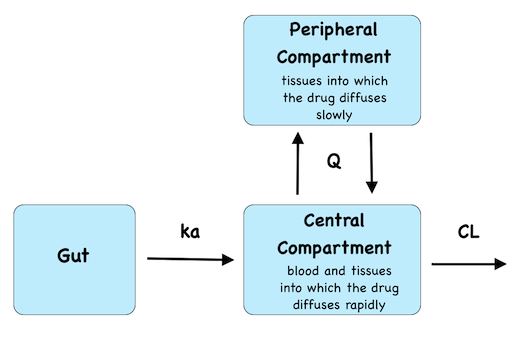
\includegraphics[width=3.5in,trim=0in 0in 0 0in]{graphics/appendix/twoCpt.png}
\caption{{Two Compartment Model: Describes the absorption of a drug in a patient's body.}}
\label{TwoCptNice}
\end{center}
\end{figure}

We describe the drug absorption using the following differential equations:

\begin{eqnarray*}
  \frac{dy_{\mathrm{gut}}}{dt} &=& -k_a y_{\mathrm{gut}} \\
  \frac{dy_{\mathrm{central}}}{dt} &=& k_a y_{\mathrm{gut}} - (\frac{CL}{V_{\mathrm{central}}} + \frac{Q}{V_{\mathrm{central}}}) y_{\mathrm{central}} +  \frac{Q}{V_{\mathrm{peripheral}}} y_{\mathrm{peripheral}} \\
\frac{dy_{\mathrm{peripheral}}}{dt} &=& \frac{Q}{V_{\mathrm{central}}} y_{\mathrm{central}} - \frac{Q}{V_{\mathrm{peripheral}}} y_{\mathrm{peripheral}}
\end{eqnarray*}

with \\  
$y_{\mathrm{gut}}$ : the drug amount in the gut (mg)  \\
$y_{\mathrm{central}}$ : the drug amount in the central compartment (mg)  \\
$y_{\mathrm{peripheral}}$ : the drug amount in the peripheral compartment (mg)  \\
$k_a$ : the rate constant at which the drug flows from the gut to the central compartment ($h^{-1}$)  \\
$Q$ : the clearance at which the drug flows back and forth between the central and the peripheral compartment (L/h) \\ 
$CL$ : the clearance at which the drug is cleared from the central compartment (L/h)  \\
$V_{\mathrm{central}}$ : the volume of the central compartment (L)  \\
$V_{\mathrm{peripheral}}$ : the volume of the peripheral compartment (L) \\

The data we fit our model to is the drug concentration in the blood, which our model treats as the concentration in the central compartment, and is given by:

$$ c = \frac{y_{\mathrm{central}}}{V_{\mathrm{central}}} $$

\subsubsection{Overview of Tools for Solving Differential Equations} \ \\ \ \\
Solving ODEs can be notoriously hard.

In the best case scenario, an ODE system has an analytical solution we can hand-code (as we have done for the one and two compartment models). The vast majority of times, we need to approximate the solution numerically. There exists a very nice technique, involving matrix exponentials, for solving linear ODEs. Nonlinear systems are significantly more difficult but fortunately we can tackle these problems with numerical integrators.

Specialized algorithms for solving ODEs tend be more efficient but have a narrower application; the reverse holds for more general tools. We provide both, thereby allowing users to tackle a broad range of problems and optimize their model when possible  (Figure~\ref{DiffEqTools}).

\begin{Figure}[!htb]
\begin{center}
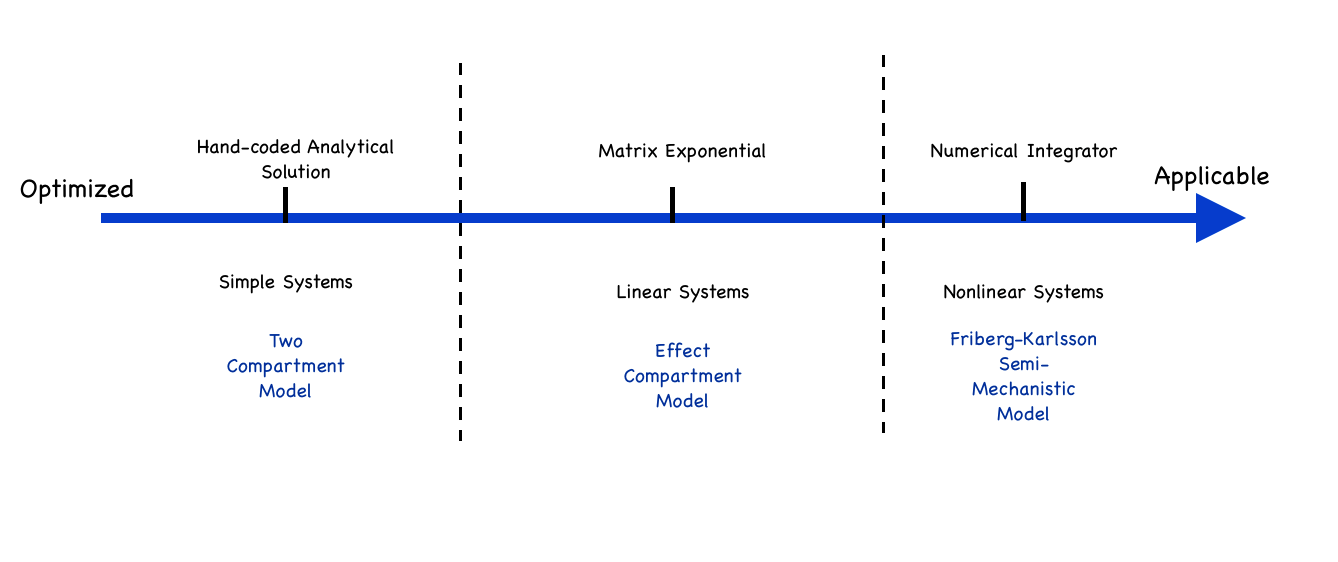
\includegraphics[width=6.5in,trim=0in 0in 0 0in]{graphics/appendix/ODEsolvers_ext.png}
\caption{{The ``Optimized-Applicable Spectrum" of tools for solving differential equations: the top line gives the technique to solve differential equations, the next line the type of ODE system this method should be applied to, and the third line (in blue) an example from pharmacometrics. We discuss these examples in greater details in sections 2 and 3 of the manual.}}
\label{DiffEqTools}
\end{center}
\end{figure}

\subsubsection{The Event Schedule} \ \\ \ \\
The ODE system only describes the natural evolution of the patient's system, that is how the drug behaves once it is already in the body. It does not account for outside interventions during the treatment, such as the intake of a drug. To be accurate, our model must compute these exterior events and solve ODEs in the context of an event schedule.

We follow the convention set by NONMEM\textregistered\footnote{NONMEM\textregistered\ is licensed and distributed by ICON Development Solutions.}, which is popular amongst pharmacometricians and which we find acceptable.

An event can either be a change in the state of the system or the measurement of a certain quantity. We distinguish two types of events:
\begin{enumerate}
  \item \textbf{State Changer}: an (exterior) intervention that alters the state of the system (for example, a bolus dosing)
  \item \textbf{Observation}: the measurement of a quantity of interest at a certain time
\end{enumerate}

Between two subsequent events, the ODEs fully describe the PKPD system. Knowing the state $y_0$ at time $t_0$ fully defines the solution at finite times. Exploiting this property, Torsten calculates amounts in each compartment from one event to the other. The initial conditions of the ODEs are specified by the previous event and the ODEs integrated from $t_{\mathrm{previous}}$ to $t_{\mathrm{current}}$.

If an event is a state changer, Torsten computes the changes in the state after integrating the ODEs.

The user passes the event schedule using a data table. NONMEM's convention allows one row to code for multiple events. For example, a single row can specify a patient receives multiple doses at a regular time interval. Consider:

\texttt{TIME = 0, EVID = 1, CMT = 1, AMT = 1500, RATE = 0, ADDL = 4, II = 10, SS = 0}

This row specifies that a time 0 (TIME = 0), a patient receives a 1500 mg (AMT = 1500) drug dose (EVID = 1) in the gut (CMT = 1), and will receive an additional dose every 10 hours (II = 10) until the patient has taken a total of 5 doses (ADDL = 4, being the number of additional doses, + 1, the original dose). Such an event really corresponds to 5 dosing events. Torsten augments the event schedule accordingly, before solving the ODEs recursively from one event to the other.

In summary, each Torsten function:
\begin{enumerate}
  \item augments the event schedule to include all state changers
  \item calculates the amounts in each compartment at each event of the augmented schedule by
  %\renewcommand{\theenumi}{\Alph{enumi}} 
  \begin{enumerate}
    \item integrating the ODEs and computing the \textit{natural} evolution of the system
    \item computing the effects of state changers
  \end{enumerate}
  \item returns the amounts at each event of the original schedule.
\end{enumerate}

\subsection{Bayesian Data Analysis with Stan} \ \\

Stan is primarily designed for bayesian data analysis. It provides users with great flexibility, both for implementing stochastic and deterministic features. This allows users to specify complex mixed-effect models, as the ones we may encounter in pharmacometrics.

Its default algorithm for full bayesian inference is the No-U-Turns Sampler (NUTS) \cite{nuts}. NUTS, an adaptative Hamiltonian Monte Carlo (HMC) \cite{HMC} algorithm, has proven more efficient than commonly used random walk Monte Carlo Markov Chains algorithms, such as Metropolis-Hastings and Gibbs sampling, for complex high-dimensional problems \cite{nuts}. Here, by ``complex" we mean a non-trivial relationship between the independent and dependent variables, such as one that involves solving ODEs and unlike one that is simply linear. The dimensionality of a model relates to the number of parameters, and scales up rapidly in hierarchical models. In pharmacometrics, this hierarchy may for instance result from modeling variability between patients or studies.

\subsubsection{Hamiltonian Monte Carlo} \ \\

The basic idea behind HMC is to treat the Markov Chain as a particle that moves in the parameter space and the posterior as a physical potential. More precisely, the potential is set to the negative of the log posterior. Instead of a random step, we give the particle a random shove or momentum. The particle accelerates when the potential decreases (i.e. when the posterior increases) and decelerates when the potential increases. We obtain this behavior by simulating the laws of classical mechanics, elegantly described by Hamilton's equations. See [?] for a more thorough introduction to HMC.

From a developer's perspective, the key consideration is we need to compute the gradient of the log posterior. Considering the gradient may have a complex expression, this is not a trivial task. Stan calculates gradients with reverse automatic differentiation. The posterior is \textit{translated} into an expression graph and the derivatives calculated by  applying the chain rule at the nodes of the graph \cite{AD}. 

\subsubsection{The \texttt{var} class} \ \\

At a C++ level, this scheme requires the use of a new class, \texttt{var}, which contains (1) the value of the variable and (2) its adjoint with respect to the log posterior\footnote{The adjoint of $x$ with respect to $f$ is the derivative of $f$ with respect to x.}. This introduces an important distinction between parameters, with respect to which we need to calculate the gradient of the log posterior and which must therefore be coded as \texttt{var}, and data, which are more simply coded as \texttt{double}.

A Stan function must be templated to allow for both \texttt{var} or \texttt{double} type arguments. At the API level, this allows the user to call the function on both parameters or data.

In addition, the chain rule must be applicable to any operation used in the function (for example addition (\texttt{+}) or multiplication (\texttt{*}), or other functions in the \texttt{Stan-math} library such as \texttt{exp} or \texttt{cos}). Alternatively, we can hand-code the jacobian\footnote{The jacobian is the generalized gradient and accounts for the case in which the output of a function contains more than one element, and its input more than one parameter.} of a function's output with respect to its input parameters. Doing the latter is often preferable, because automatic differentiation is an approximation and can be computationally costly. If the jacobian is known, we gain much by hand-coding it. 


\subsection{Solving Differential Equations in Stan's Geometrical Framework} \ \\

We need to solve differential equations and compute the Jacobian of the solutions with respect to the parameters. 

\subsection{C++ Implementation} \ \\ \ \\
The only thing that distinguishes two Torsten functions is the method they use to solve ODEs (i.e.s task (2)(a) of the above list). This structural scheme allows us to take advantage of the object-oriented nature of C++. All Torsten functions call the same procedure, \texttt{pred}, which predicts the amounts. In the process \texttt{pred} calls the specialized procedure, \texttt{pred1}, to solve the ODEs, i.e. perform task (2)(a).

Rather than using a simple function, we define \texttt{pred1\_structure}, a functor or structure of functions. Each Torsten function constructs a \texttt{pred1\_structure} object and determines the ODE solver.

\fi
%%%%%%%%%%%%%%%%%%%%%%%%%%%%%%%%%%%%%%%%%%%%%%%%%%%%%%%%%%%%%%%%%%%%%%%%

\subsection{Implementing Torsten} \ \\ \ \\
Stan's \texttt{math} library is written in C++, which offers a great deal of speed and flexibility. The Stan language provides a very handy interface that allows us to focus on statistical modeling and saves us the trouble of doing extensive coding in C++. At run time, a \textit{make} file translates our Stan model into C++, which then gets compiled and executed. Accordingly, there are two steps to add a function to Stan: (1) write the procedure in C++, (2) expose the procedure to the language so users may use it in a Stan file.

The Stan code is open-source and available on GitHub. It is compartmentalized into several repos: \texttt{math} contains the mathematical functions, \texttt{Stan} exposes these functions. Other repos provide code to interface Stan with higher level languages, such as R and Python. Torsten exists as a forked version of \texttt{math} and \texttt{Stan}. Other repos remain unchanged.

Regularly, we merge Stan's latest release into Torsten.

\subsubsection*{Modifications in math}
All Torsten files are located in the \texttt{Torsten} directory, under \texttt{stan/math}. The code can be found on GitHub: \url{https://github.com/metrumresearchgroup/math} 

\subsubsection*{Modifications in Stan}
We do further modifications in \texttt{Stan} to expose Torsten's functions. We edit \texttt{function\_signatures.h} to expose \texttt{PKModelOneCpt}, \texttt{PKModelTwoCpt}, and \texttt{linOdeModel}. The general ODE model functions are higher-order functions (i.e. they take another function as one of their arguments). They are exposed by directly modifying the grammar files, following closely the example of \texttt{integrate\_ode\_rk45} and \texttt{integrate\_ode\_bdf}.

The code can be found on GitHub:  \url{https://github.com/metrumresearchgroup/stan}.

\bibliographystyle{custom}
\bibliography{alpha,custom}


\end{document}
